% !TEX TS-program = xelatex
% !TeX spellcheck = ru_RU
% !TEX root = egraphs_talk.tex
% !BIB program = bibtex

\documentclass[aspectratio=169
  %, draft      % speedup compilation
  %, handout    % eliminate pauses
  , xcolor={svgnames}
  , russian  % This line affects translation of theorem titles
  ]{beamer}

%%%%%%%%%%%%%%%%%%%%%%%%%%%%%%%%%%%%%%%%
\makeatletter
\@ifclassloaded{beamer}{
  \usefonttheme{professionalfonts}
  \usepackage[svgnames]{xcolor}
  \usetheme{CambridgeUS}
  \setbeamertemplate{enumerate items}[circle]
  % get rid of header navigation bar
  \setbeamertemplate{headline}{}
  % get rid of bottom navigation symbols
  \setbeamertemplate{navigation symbols}{}
  % get rid of footer
  %\setbeamertemplate{footline}{}
  \setbeamertemplate{section in toc} {\inserttocsectionnumber.~\inserttocsection}
  \institute{матмех}

  \titlegraphic{
        \hspace{5cm}
        {\tiny Дата сборки: \today}
        \hspace{1.8cm}
    \includegraphics[scale=.8]{../by.eps}
  }
%  \addtobeamertemplate{title page}{}{
%    \begin{center}
%        {\tiny Дата сборки: \today}
%    \end{center}
%  }
}
{}
\makeatother
%%%%%%%%%%%%%%%%%%%%%%%%%%%%%%%%%%%%%%%%%%%%%
\usepackage{ifxetex,ifluatex}
\newif\ifxetexorluatex
    \ifxetex
        \xetexorluatextrue
    \else
        \ifluatex
            \xetexorluatextrue
        \else
            \xetexorluatexfalse
        \fi
    \fi


\author{Аверин Павел}

\ifxetexorluatex
    \usepackage{fontspec}
%    \usepackage{unicode-math} % Allow TTF and OTF fonts in math and allow direct typing unicode math characters.
    \usepackage{euler-math}
    %\setmainfont[Ligatures=TeX]{CMU Serif}
    %\setsansfont[Ligatures=TeX]{CMU Sans Serif}
    \setmainfont[Ligatures=TeX]{Liberation Serif}
    \setsansfont[Ligatures=TeX]{Liberation Sans}
%    \setmathfont{Latin Modern Math}
%    \setmathfont{NotoSansMath-Regular.ttf}
%    \setmathfont{FiraMath-Regular.otf} % from texlive-fonts-extra
%    \setmathfont{TeX Gyre Pagella Math} % Doesn't have \setminus
%    \setmathfont[Scale=MatchUppercase]{Asana Math}
%    \setmainfont{TeX Gyre Bonum}
%    \setmathfont{TeX Gyre Bonum Math}
%\setmonofont{Fira Code}[Contextuals=AlternateOff,Ligatures=Common]
%\setmonofont{Fira Code}[Contextuals=Alternate,Scale=0.9]
    \setmonofont{Monaco for Powerline}[Scale=0.9]
    %\setmonofont{Latin Modern Mono}[Scale=1]

    \usepackage{polyglossia}
    \setmainlanguage{russian}
    \setotherlanguage{english}
\else
    \usepackage[utf8]{inputenc}
    \usepackage[T2A]{fontenc}
    \usepackage[russian,english]{babel}
    \usepackage{euler}
    %\usepackage{lmodern}
\fi
\usepackage{movie15}
\usepackage{fontawesome}
% \newfontfamily{\FA}{Font Awesome 5 Free} % some glyphs missing
\expandafter\def\csname faicon@facebook\endcsname{{\FA\symbol{"F09A}}}
\def\faQuestionSign{{\FA\symbol{"F059}}}
\def\faQuestion{{\FA\symbol{"F128}}}
\def\faExclamation{{\FA\symbol{"F12A}}}
\def\faUploadAlt{{\FA\symbol{"F093}}}
\def\faLemon{{\FA\symbol{"F094}}}
\def\faPhone{{\FA\symbol{"F095}}}
\def\faCheckEmpty{{\FA\symbol{"F096}}}
\def\faBookmarkEmpty{{\FA\symbol{"F097}}}

\newcommand{\faGood}{\textcolor{ForestGreen}{\faThumbsUp}}
\newcommand{\faBad}{\textcolor{red}{\faThumbsODown}}
\newcommand{\faWrong}{\textcolor{red}{\faTimes}}
\newcommand{\faMaybe}{\textcolor{blue}{\faQuestion}}
\newcommand{\faCheckGreen}{\textcolor{ForestGreen}{\faCheck}}
%%%%%%%%%%%%%%%%%%%%%%%%%%%%%%%%%%%%%%%%%%%%%
% https://latex.org/forum/viewtopic.php?t=34345
\usepackage[backend=biber,sorting=none]{biblatex}

\makeatletter
\@ifclassloaded{beamer}{
    %% Set the icons
    \setbeamertemplate{bibliography item}{%
    \ifboolexpr{ test {\ifentrytype{book}} or test {\ifentrytype{mvbook}}
      or test {\ifentrytype{collection}} or test {\ifentrytype{mvcollection}}
      or test {\ifentrytype{reference}} or test {\ifentrytype{mvreference}} }
      {\setbeamertemplate{bibliography item}[book]}
      {\ifentrytype{online}
        {\setbeamertemplate{bibliography item}[online]}
        {\setbeamertemplate{bibliography item}[article]}}%
    \usebeamertemplate{bibliography item}}

    \defbibenvironment{bibliography}
    {\list{}
       {\settowidth{\labelwidth}{\usebeamertemplate{bibliography item}}%
        \setlength{\leftmargin}{\labelwidth}%
        \setlength{\labelsep}{\biblabelsep}%
        \addtolength{\leftmargin}{\labelsep}%
        \setlength{\itemsep}{\bibitemsep}%
        \setlength{\parsep}{\bibparsep}}}
    {\endlist}
    {\item}
     % http://codydunne.blogspot.com/2012/01/suppressing-bibtex-fields-for-specific.html
     \AtEveryBibitem{% Clean up the bibtex rather than editing it
     \clearlist{address}
     \clearfield{booktitle}
     \clearfield{date}
     \clearfield{doi}
     \clearname{editor}
     \clearfield{eprint}
     \clearfield{isbn}
     \clearfield{issn}
     \clearlist{location}
     \clearfield{month}
     \clearfield{pages}
     \clearlist{publisher}
     \clearfield{series}
    }
}
{}
\makeatother
%%%%%%%%%%%%%%%%%%%%
\usepackage{relsize} % \mathlarger{..}
\usepackage{hyperref}
\hypersetup{colorlinks,citecolor={blue},linkcolor=blue,urlcolor=DarkBlue}


%%%%%%%%%%%%%%%%%%%%%%%%%%%%%%%%%%%%%%%%%%%%%%%5
\usepackage{soul} % for \st that strikes through
\usepackage[normalem]{ulem} % \sout

\usepackage{stmaryrd}
\newcommand{\sem}[1]{\ensuremath{\llbracket #1\rrbracket}}

% We should use the following commands as \ocaml{} to prevent chewing
% extra space
\newcommand{\Linux}{\textsc{Linux}}
\newcommand{\ocaml}{\textsc{OCaml}}
\newcommand{\OCaml}{\ocaml}
\newcommand{\haskell}{\textsc{Haskell}}
\newcommand{\Haskell}{\haskell}
\newcommand{\Rust}{\textsc{Rust}}
\newcommand{\Coq}{\textsc{Coq}}
\newcommand{\Java}{\textsc{Java}}
\newcommand{\CXX}{\textsc{C++}}
\newcommand{\Scheme}{\textsc{Scheme}}
\newcommand{\Kotlin}{\textsc{kotlin}}
\newcommand{\CSharp}{\textsc{C\#}}




%\let\thefootnote\relax\footnotetext{Put your text here}
\DeclareMathOperator{\arr}{\rightarrow}

%%%%%%%%%%%%%%%%%%%%%%%%%%%%%%%%%%%%%%%%%%%%%%%%%%%%%%%%%%%
\usepackage{tikz}
\usetikzlibrary{cd}
\usepackage{tikz-cd}
\usepackage{caption}
\usepackage{subcaption}





\usepackage[useregional]{datetime2}
% https://tex.stackexchange.com/a/132994/171947
\usepackage{amsthm}
\newtheorem{exercise}[theorem]{Упражнение}

\ifxetexorluatex
\else
\patchcmd{\definition}{Definition}{Определение}{}{}
\fi

\usepackage{scalerel}
\DeclareMathOperator*{\myvee}{\scalerel*{\vee}{\sum}}
\DeclareMathOperator*{\mywedge}{\scalerel*{\wedge}{\sum}}

\usepackage{array}
\usepackage{makecell}
%\newcolumntype{MC}[1]{>{\centering\arraybackslash}p{#1}}
%
%\usepackage{tabulary}
% https://tex.stackexchange.com/questions/380799/warning-when-adding-package-minted
\usepackage[autostyle]{csquotes}
\ifxetexorluatex
\else
% https://tex.stackexchange.com/a/377117/171947
\renewcommand\thempfootnote{\alph{mpfootnote}}
\fi


% color options
\definecolor{YellowGreen} {HTML}{B5C28C}
\definecolor{ForestGreen} {HTML}{009B55}
\definecolor{MyPurple}{HTML}{7f007f}
\definecolor{CommentColor}{HTML}{3f7f5f}
\def\HaskellTypeclassColor\PYG{k+kt}
\def\HaskellCommentColor\PYG{c+c1}

\newif\ifminted
\newif\iflistings

\listingstrue
%\mintedtrue

\iflistings
    \usepackage{listings}
    %\input{../ss24/riscv-asm.tex}
    %\newcommand{\inline}[1]{\lstinline{haskell}{#1}}
    % TODO: https://tex.stackexchange.com/questions/4198/emphasize-word-beginning-with-uppercase-letters-in-code-with-lstlisting-package
    \definecolor{eclipseGreen}{RGB}{63,127,95}

    % https://tex.stackexchange.com/a/4199
    \makeatletter
    \newcommand*\ocamlidstyle{%
            \expandafter\id@style\the\lst@token\relax
    }
    \def\id@style#1#2\relax{%
            \ifcat#1\relax\else
                    \ifnum`#1=\uccode`#1%
                             \ttfamily\bfseries\color{MyPurple}
                    \else
                                                \ttfamily
                    \fi
            \fi
    }
    \makeatother

    \lstdefinelanguage{none}{ identifierstyle= }
    \lstdefinelanguage{menhir}
      { identifierstyle=
      , morecomment=[s]{/*}{*/}
      , commentstyle=\color{eclipseGreen} % style of comments
      , classoffset=0
      , keywords={ left, nonassoc, start,  token, type
      }
      , keywordstyle=\ttfamily\bfseries\color{MyPurple}
    }
    \lstdefinelanguage{ocamllex}
      { identifierstyle=
      , morecomment=[s]{/*}{*/}
      , commentstyle=\color{eclipseGreen} % style of comments
      , classoffset=0
      , keywords={ and, rule, parsem if, then, else, eof, as, raise, parse
      }
      , keywordstyle=\ttfamily\bfseries\color{MyPurple}
      , stringstyle=\color{blue}
      , morestring=*[d]{"}
      , morestring=*[d]{'}
    }
    \ifxetexorluatex
    \lstdefinelanguage{ocaml}{
        basicstyle=\ttfamily   % Вот тут надо стиль ставить, а не у идентификаторов
        %, identifierstyle=\ocamlidstyle
        , identifierstyle=\ttfamily
        %, commentstyle=\HaskellCommentColor\itshape\HaskellCommentColor
        , sensitive=true
        %
        , classoffset=0
        , keywords={ fun, function, and, let, rec, in, match, with, when
            , class, type, of, do, done, as, val
            , inherit, module, struct, sig, include
            , if, then, else, while
            , try, exception, raise
            , mod
            , assert, true, false, begin, end, lazy
            , @@deriving
            , Some, None
        }
        , keywordstyle=\ttfamily\bfseries\color{MyPurple} %\underbar
        , classoffset=1
        , morekeywords={pure,empty,select,branch,oneOf}
        , keywordstyle=\color{MyPurple}
        , classoffset=2
        , morekeywords={Monad,Applicative,Selective,String
            ,Either,Left,Right
            ,Maybe,Some,None
        }
        , keywordstyle=\ttfamily\bfseries\color{MyPurple}
        , classoffset=0,
        %keywordstyle=[2]{\color{orange}},
        otherkeywords={::},
        %identifierstyle=\fontfamily{cmtt}\selectfont\ttfamily,
        %basewidth={0.5em,0.5em},
        columns=fixed,
        %fontadjust=true,
        %literate={->}{{$\to$}}3 {===}{{$\equiv$}}1 {=/=}{{$\not\equiv$}}1 {|>}{{$\triangleright$}}3 {\\/}{{$\vee$}}2 {/\\}{{$\wedge$}}2 {>=}{{$\ge$}}1 {<=}{{$\le$}} 1,
        , morecomment=[s]{(*}{*)}
        , commentstyle=\color{eclipseGreen} % style of comments
        %, literate={\$}{{\textcolor{blue}{\$}}}1
        %, literate={<\$>}{{\textcolor{RawSienna}{\ <\$>\ } }}1
        %           {>?>}{{\textcolor{RawSienna}{\ >?>\ } }}1
        , string = [d]{"}
        , showstringspaces=false
        , stringstyle = \color{black}
        %, morestring = [d][\color{orange}]{'}
        %, moredelim={[s][\color{orange}\ttfamily]{'}{'}}
    }
    \else
        \lstdefinelanguage{ocaml}{
            % modified minial style for pdflatex
            basicstyle=\ttfamily
            , identifierstyle=\ttfamily
            , sensitive=true
            , classoffset=0
            , extendedchars=true
            , literate=
                {а}{{a}}1 {б}{{b}}1 {в}{{v}}1 {г}{{g}}1 {д}{{d}}1
                {е}{{e}}1 {ё}{{e}}1 {ж}{{zh}}1 {з}{{z}}1 {и}{{i}}1 {й}{{j}}1
                       {к}{{k}}1 {л}{{l}}1 {м}{{m}}1 {н}{{n}}1 {о}{{o}}1
                       {п}{{p}}1 {р}{{r}}1 {с}{{s}}1 {т}{{t}}1 {у}{{u}}1
                       {ф}{{f}}1 {х}{{h}}1 {ц}{{ts}}1 {ч}{{ch}}1 {ш}{{sh}}1
                       {щ}{{sch}}1 {ъ}{{}}1 {ы}{{y}}1 {ь}{{}}1 {э}{{e}}1
                       {ю}{{u}}1  {я}{{a}}1
                {А}{{a}}1 {Б}{{b}}1 {В}{{v}}1 {Г}{{g}}1 {Д}{{d}}1
                {Е}{{e}}1 {Ё}{{e}}1 {Ж}{{zh}}1 {З}{{z}}1 {И}{{i}}1
                {Й}{{j}}1 {К}{{k}}1 {Л}{{l}}1 {М}{{m}}1 {Н}{{n}}1
                {О}{{o}}1 {П}{{p}}1 {Р}{{r}}1 {С}{{s}}1 {Т}{{t}}1
                {У}{{u}}1 {Ф}{{f}}1 {х}{{h}}1 {ц}{{ts}}1 {Ч}{{ch}}1
                {Ш}{{sh}}1 {Щ}{{sch}}1 {Ъ}{{}}1 {Ы}{{y}}1 {Ь}{{}}1
                {Э}{{e}}1 {Ю}{{u}}1  {Я}{{a}}1
            , keywords={ fun, function, and, let, rec, in, match, with, when
                , class, type, of, do, done, as, val
                , inherit, module, struct, sig, include
                , if, then, else, while
                , try, exception, raise
                , mod
                , assert, true, false, begin, end, lazy
                , @@deriving
                , Some, None
            }
            , keywordstyle=\ttfamily\bfseries\color{MyPurple} %\underbar
            , morecomment=[s]{(*}{*)}
            , commentstyle=\color{eclipseGreen} % style of comments
            , string = [d]{"}
            , showstringspaces=false
            , stringstyle = \color{black}
            %, moredelim={[s][\color{eclipseGreen}\ttfamily]{'}{'}}
        }
    \fi
    \lstset{ language=ocaml }
    \lstnewenvironment{mlisting}[1][]{\lstset{inputencoding=latin1, language=ocaml,#1}%
    }{%
    }

    \lstdefinelanguage{csharp}
      { basicstyle=\ttfamily   % Вот тут надо стиль ставить, а не у идентификаторов
      , identifierstyle=\ttfamily
      , sensitive=true
      , keywords={ new, var, in, foreach }
      , keywordstyle=\ttfamily\bfseries\color{MyPurple}
      , commentstyle=\color{eclipseGreen}
      , morecomment=[f][\color{eclipseGreen}][0]{//},
      }


% https://github.com/cansik/kotlin-latex-listing
\lstdefinelanguage{Kotlin}{
  comment=[l]{//},
  commentstyle={\color{gray}\ttfamily},
  emph={filter, first, firstOrNull, forEach, lazy, map, mapNotNull, println},
  emphstyle={\color{OrangeRed}},
  identifierstyle=\color{black},
  keywords={!in, !is, abstract, actual, annotation, as, as?, break, by, catch, class, companion, const, constructor, continue, crossinline, data, delegate, do, dynamic, else, enum, expect, external, false, field, file, final, finally, for, fun, get, if, import, in, infix, init, inline, inner, interface, internal, is, lateinit, noinline, null, object, open, operator, out, override, package, param, private, property, protected, public, receiveris, reified, return, return@, sealed, set, setparam, super, suspend, tailrec, this, throw, true, try, typealias, typeof, val, var, vararg, when, where, while},
  keywordstyle={\color{MyPurple}\bfseries},
  morecomment=[s]{/*}{*/},
  morestring=[b]",
  morestring=[s]{"""*}{*"""},
  ndkeywords={@Deprecated, @JvmField, @JvmName, @JvmOverloads, @JvmStatic, @JvmSynthetic, Array, Byte, Double, Float, Int, Integer, Iterable, Long, Runnable, Short, String, Any, Unit, Nothing},
  ndkeywordstyle={\color{MyPurple}\bfseries},
  sensitive=true,
  stringstyle={\color{ForestGreen}\ttfamily},
}

    %\def\mlinline[1]{\lstinline[langauge=ocaml]{#1}} % is not possible

    \lstdefinelanguage{Kotlin}{
      comment=[l]{//},
      commentstyle={\color{gray}\ttfamily},
      emph={filter, first, firstOrNull, forEach, lazy, map, mapNotNull, println},
      emphstyle={\color{blue}},
      identifierstyle=\color{black},
      keywords={!in, !is, abstract, actual, annotation, as, as?, break, by, catch, class, companion, const, constructor, continue, crossinline, data, delegate, do, dynamic, else, enum, expect, external, false, field, file, final, finally, for, fun, get, if, import, in, infix, init, inline, inner, interface, internal, is, lateinit, noinline, null, object, open, operator, out, override, package, param, private, property, protected, public, receiveris, reified, return, return@, sealed, set, setparam, super, suspend, tailrec, this, throw, true, try, typealias, typeof, val, var, vararg, when, where, while},
      keywordstyle={\color{blue}\bfseries},
      morecomment=[s]{/*}{*/},
      morestring=[b]",
      morestring=[s]{"""*}{*"""},
      ndkeywords={@Deprecated, @JvmField, @JvmName, @JvmOverloads, @JvmStatic, @JvmSynthetic, Array, Byte, Double, Float, Int, Integer, Iterable, Long, Runnable, Short, String, Any, Unit, Nothing},
      ndkeywordstyle={\color{blue}\bfseries},
      sensitive=true,
      stringstyle={\color{ForestGreen}\ttfamily},
    }
    \ifpdftex
        \usepackage{etoolbox}
        \expandafter\patchcmd\csname \string\lstinline\endcsname{%
            \leavevmode
            \bgroup
        }{%
            \leavevmode
            \ifmmode\hbox\fi
            \bgroup
        }{}{%
            \typeout{Patching of \string\lstinline\space failed!}%
        }
    \fi
\fi

\ifminted
    \usepackage[cache=true]{minted}
    \usemintedstyle{perldoc}
    \def\hsinline{\mintinline{haskell}}
    \def\mlinline{\mintinline[escapeinside=||]{ocaml}}

%\def\hsinline{\mintinline{haskell}}
%\def\inline{\hsinline}
\fi


\usepackage{tikz} % Мощный пакет для создание рисунков, однако может очень сильно замедлять компиляцию
\usetikzlibrary{decorations.pathreplacing,calc,shapes,positioning,tikzmark}
\newcounter{tmkcount}

\tikzset{
    use tikzmark/.style={
        remember picture,
        overlay,
        execute at end picture={
            \stepcounter{tmkcount}
        },
    },
    tikzmark suffix={-\thetmkcount}
}
%\newcommand\centerarc{} % just for safety
\def\tikzHighlight(#1)(#2){
  \draw[fill=gray,opacity=0.1]
    ([shift={(-3pt,2ex)}]pic cs:#1)
    rectangle
    ([shift={(3pt,-0.65ex)}]pic cs:#2);
}


\renewcommand{\epsilon}{\varepsilon}
\renewcommand{\theta}{\vartheta}
\renewcommand{\kappa}{\varkappa}
\renewcommand{\rho}{\varrho} % remember my teacher and friend Adalberto!
\renewcommand{\phi}{\varphi} % TODO(Kakadu): sometimes we need to repeat it in the beginning of the slide


% For every picture that defines or uses external nodes, you'll have to
% apply the 'remember picture' style. To avoid some typing, we'll apply
% the style to all pictures.
\tikzstyle{every picture}+=[remember picture]

% By default all math in TikZ nodes are set in inline mode. Change this to
% displaystyle so that we don't get small fractions.
\everymath{\displaystyle}

\bibliography{egraphs_talk.bib}
%%%%%%%%%%%%%%%%%%%%%%%%%%%%%%%%%%%%%%%%
\title[E-Graphs]{E-Graphs. Их применение в компиляторах и не только}
\date{\DTMDate{2024-09-28}}

\definecolor{ForestGreen} {HTML}{009B55}
\AtBeginSection[]
{
  \begin{frame}<beamer>
    \frametitle{Оглавление}
    \tableofcontents[currentsection,currentsubsection]
  \end{frame}
}

\usepackage{amsmath}
\usepackage{tikz}
\usepackage{xcolor}
\usepackage{multicol}
\usepackage{graphicx}
\usepackage{animate}
% in preamble

% in documenet
\usepackage{xmpmulti}
\begin{document}
\maketitle


\begin{frame}{Переписывание выражений}

    \only<1>
{
\centering

% Main expression in the middle
\Huge
\text{$(a\; *\; 2)\; /\; 2\rightarrow$ $a$}

\vspace{1cm}


}

    \only<2>
{
\centering

% Main expression in the middle
\Huge
\text{$(a\; *\; 2)\; /\; 2\rightarrow$ $a$}

\vspace{1cm}

% "Rewrite it" below the main expression
\Large
\text{Как переписать?}

\vfill

}

    \only<3>
{
\centering

% Main expression in the middle
\Huge
\text{$(a\; *\; 2)\; /\; 2\rightarrow$ $a$}

\vspace{1cm}

% "Rewrite it" below the main expression
\Large
\text{Как переписать?}

\vfill

% Columns for b1 and b2
\begin{multicols}{2}
    \textcolor{ForestGreen}{Полезные правила переписывания}
    \begin{itemize}
        \item $(x\; * \;y) \;/ \;z \;= \;x\; * \;(y \;/ \;z)$
        \item $x \; / \; x \; = \; 1$
        \item $x \; * \; 1 \; = \; x$
    \end{itemize}

    \columnbreak

    {\fontsize{13.1}{12}\selectfont \textcolor{red}{Бесполезные правила переписывания}}
    \begin{itemize}
        \item $x\; * \;2 \; = \;  x \; << \; 1$
        \item $x \;*\; y \;= \;y \;* \;x$
        \item $x \;= \;x \;* \;1$
    \end{itemize}
\end{multicols}
}
\end{frame}

\begin{frame}{Переписывание выражений. Happy path}

    \only<1>
{
    \Huge{ \centering
    $(a \; *\; 2)\; / \;2$
    }

    \vspace{1cm} % Adds some space between the expression and the bullet list

    {\fontsize{16.1}{12}\selectfont \textcolor{green}{Полезные правила переписывания}}
    {\fontsize{16.1}{12}\selectfont % Adjust the font size here
    \begin{itemize}
        \item $(x\; * \;y) \;/ \;z \;= \;x\; * \;(y \;/ \;z)$
        \item $x \; / \; x \; = \; 1$
        \item $x \; * \; 1 \; = \; x$
    \end{itemize}
    }
}

    \only<2>
{
    \Huge{ \centering
    $(a \; *\; 2)\; / \;2 \rightarrow a \;*\; (2\; /\; 2)$
    }

    \vspace{1cm} % Adds some space between the expression and the bullet list

    {\fontsize{16.1}{12}\selectfont \textcolor{ForestGreen}{Полезные правила переписывания}}
    {\fontsize{16.1}{12}\selectfont % Adjust the font size here
    \begin{itemize}
        \item $(x\; * \;y) \;/ \;z \;= \;x\; * \;(y \;/ \;z)$
        \item $x \; / \; x \; = \; 1$
        \item $x \; * \; 1 \; = \; x$
    \end{itemize}
    }
}

    \only<3>
{
    \Huge{ \centering
    $(a \; *\; 2)\; / \;2 \rightarrow a \;*\; (2\; /\; 2) \rightarrow a \;*\; 1$
    }

    \vspace{1cm} % Adds some space between the expression and the bullet list

    {\fontsize{16.1}{12}\selectfont \textcolor{ForestGreen}{Полезные правила переписывания}}
    {\fontsize{16.1}{12}\selectfont % Adjust the font size here
    \begin{itemize}
        \item $(x\; * \;y) \;/ \;z \;= \;x\; * \;(y \;/ \;z)$
        \item $x \; / \; x \; = \; 1$
        \item $x \; * \; 1 \; = \; x$
    \end{itemize}
    }
}

    \only<4>
{
    \Huge{ \centering
    $(a \; *\; 2)\; / \;2 \rightarrow a \;*\; (2\; /\; 2) \rightarrow a \;*\; 1 \rightarrow a$
    }

    \vspace{1cm} % Adds some space between the expression and the bullet list

    {\fontsize{16.1}{12}\selectfont \textcolor{ForestGreen}{Полезные правила переписывания}}
    {\fontsize{16.1}{12}\selectfont % Adjust the font size here
    \begin{itemize}
        \item $(x\; * \;y) \;/ \;z \;= \;x\; * \;(y \;/ \;z)$
        \item $x \; / \; x \; = \; 1$
        \item $x \; * \; 1 \; = \; x$
    \end{itemize}
    }
}
\end{frame}

\begin{frame}{Переписывание выражений. Проблемные случаи}

    \only<1>
{
    \LARGE{ \centering
    $(a \; *\; 2)\; / \;2 \rightarrow (a \;<<\; 1) \;/ \;2 \rightarrow \textcolor{red}{\Huge \times}$
    } \newline \newline

    \vspace{1cm} % Adds some space between the expression and the bullet list

    {\fontsize{15.1}{12}\selectfont \textcolor{red}{Бесполезные правила переписывания}}
    {\fontsize{16.1}{12}\selectfont % Adjust the font size here
    \begin{itemize}
        \item $x\; * \;2 \; = \;  x \; << \; 1$
        \item $x \;*\; y \;= \;y \;* \;x$
        \item $x \;= \;x \;* \;1$
    \end{itemize}
    }
}

\only<2>
{
    \LARGE{ \centering
    $(a \; *\; 2)\; / \;2 \rightarrow (a \;<<\; 1) \;/ \;2 \rightarrow \textcolor{red}{\Huge \times}$
    } \newline \newline
    \LARGE{ \centering
    $\textcolor{blue}{(a \;*\; 2) \;/\; 2} \rightarrow (2 \;*\; a) \;/\; 2 \rightarrow \textcolor{blue}{(a \;*\; 2) \;/\; 2}$
    }

    \vspace{1cm} % Adds some space between the expression and the bullet list

    {\fontsize{15.1}{12}\selectfont \textcolor{red}{Бесполезные правила переписывания}}
    {\fontsize{16.1}{12}\selectfont % Adjust the font size here
    \begin{itemize}
        \item $x\; * \;2 \; = \;  x \; << \; 1$
        \item $x \;*\; y \;= \;y \;* \;x$
        \item $x \;= \;x \;* \;1$
    \end{itemize}
    }
}

\only<3>
{
    \LARGE{ \centering
    $(a \; *\; 2)\; / \;2 \rightarrow (a \;<<\; 1) \;/ \;2 \rightarrow \textcolor{red}{\Huge \times}$
    } \newline \newline
    \LARGE{ \centering
    $\textcolor{blue}{(a \;*\; 2) \;/\; 2} \rightarrow (2 \;*\; a) \;/\; 2 \rightarrow \textcolor{blue}{(a \;*\; 2) \;/\; 2}$
    } \newline \newline
    \LARGE{ \centering
    $a \rightarrow a \; * \; 1 \rightarrow a \; * \; 1 \;*\; 1 \rightarrow .\;.\;.$
    }

    \vspace{1cm} % Adds some space between the expression and the bullet list

    {\fontsize{15.1}{12}\selectfont \textcolor{red}{Бесполезные правила переписывания}}
    {\fontsize{16.1}{12}\selectfont % Adjust the font size here
    \begin{itemize}
    \item $x\; * \;2 \; = \;  x \; << \; 1$
    \item $x \;*\; y \;= \;y \;* \;x$
    \item $x \;= \;x \;* \;1$
    \end{itemize}
    }
}
\end{frame}

\begin{frame}{Решение проблемы 1/3}
  \only<1>
    {
        \centering
        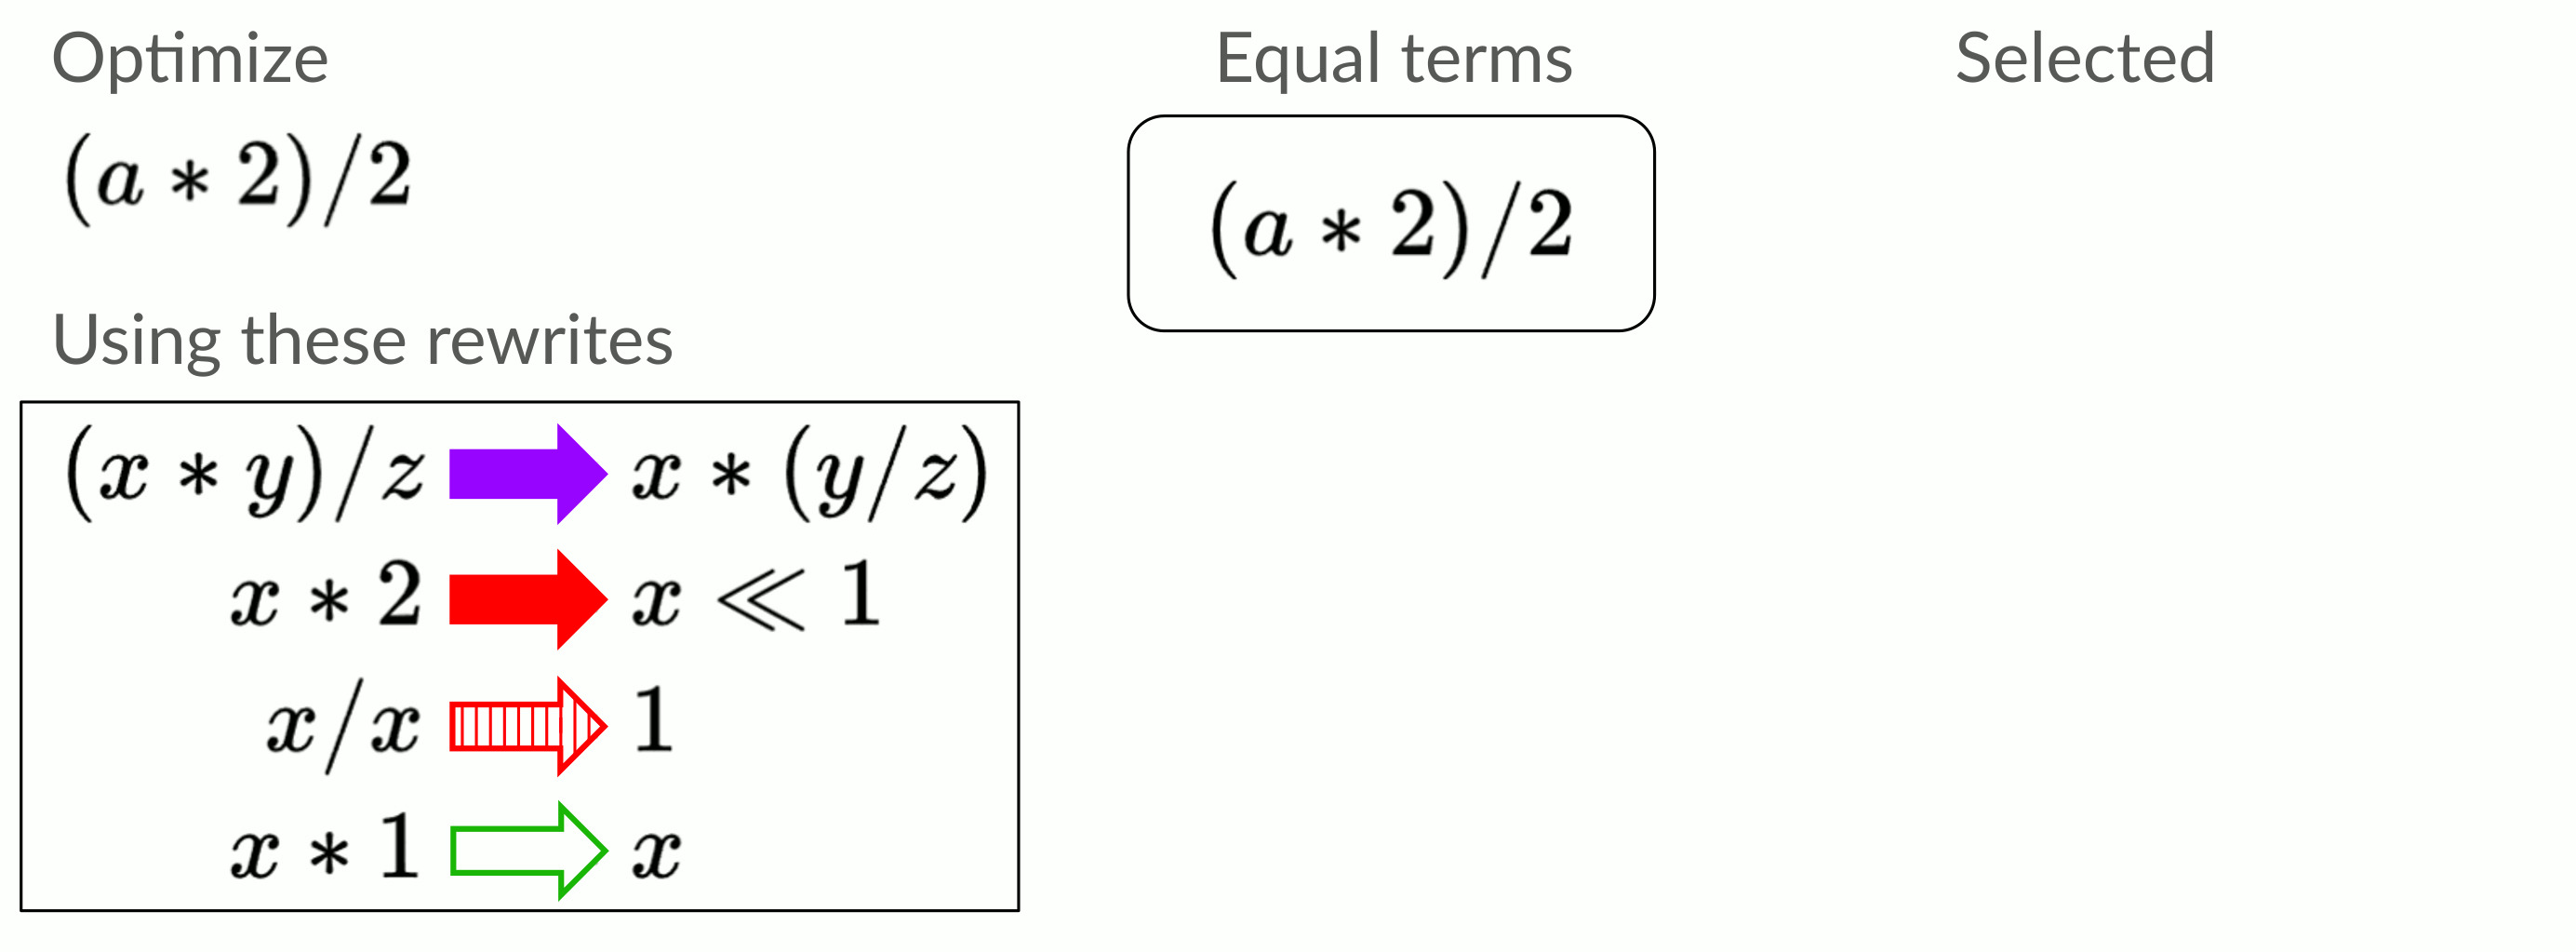
\includegraphics[width=13cm, height=5cm]{misc/egraphs_images/naive/n-0.jpg}
   }
   \only<2>
    {
        \centering
        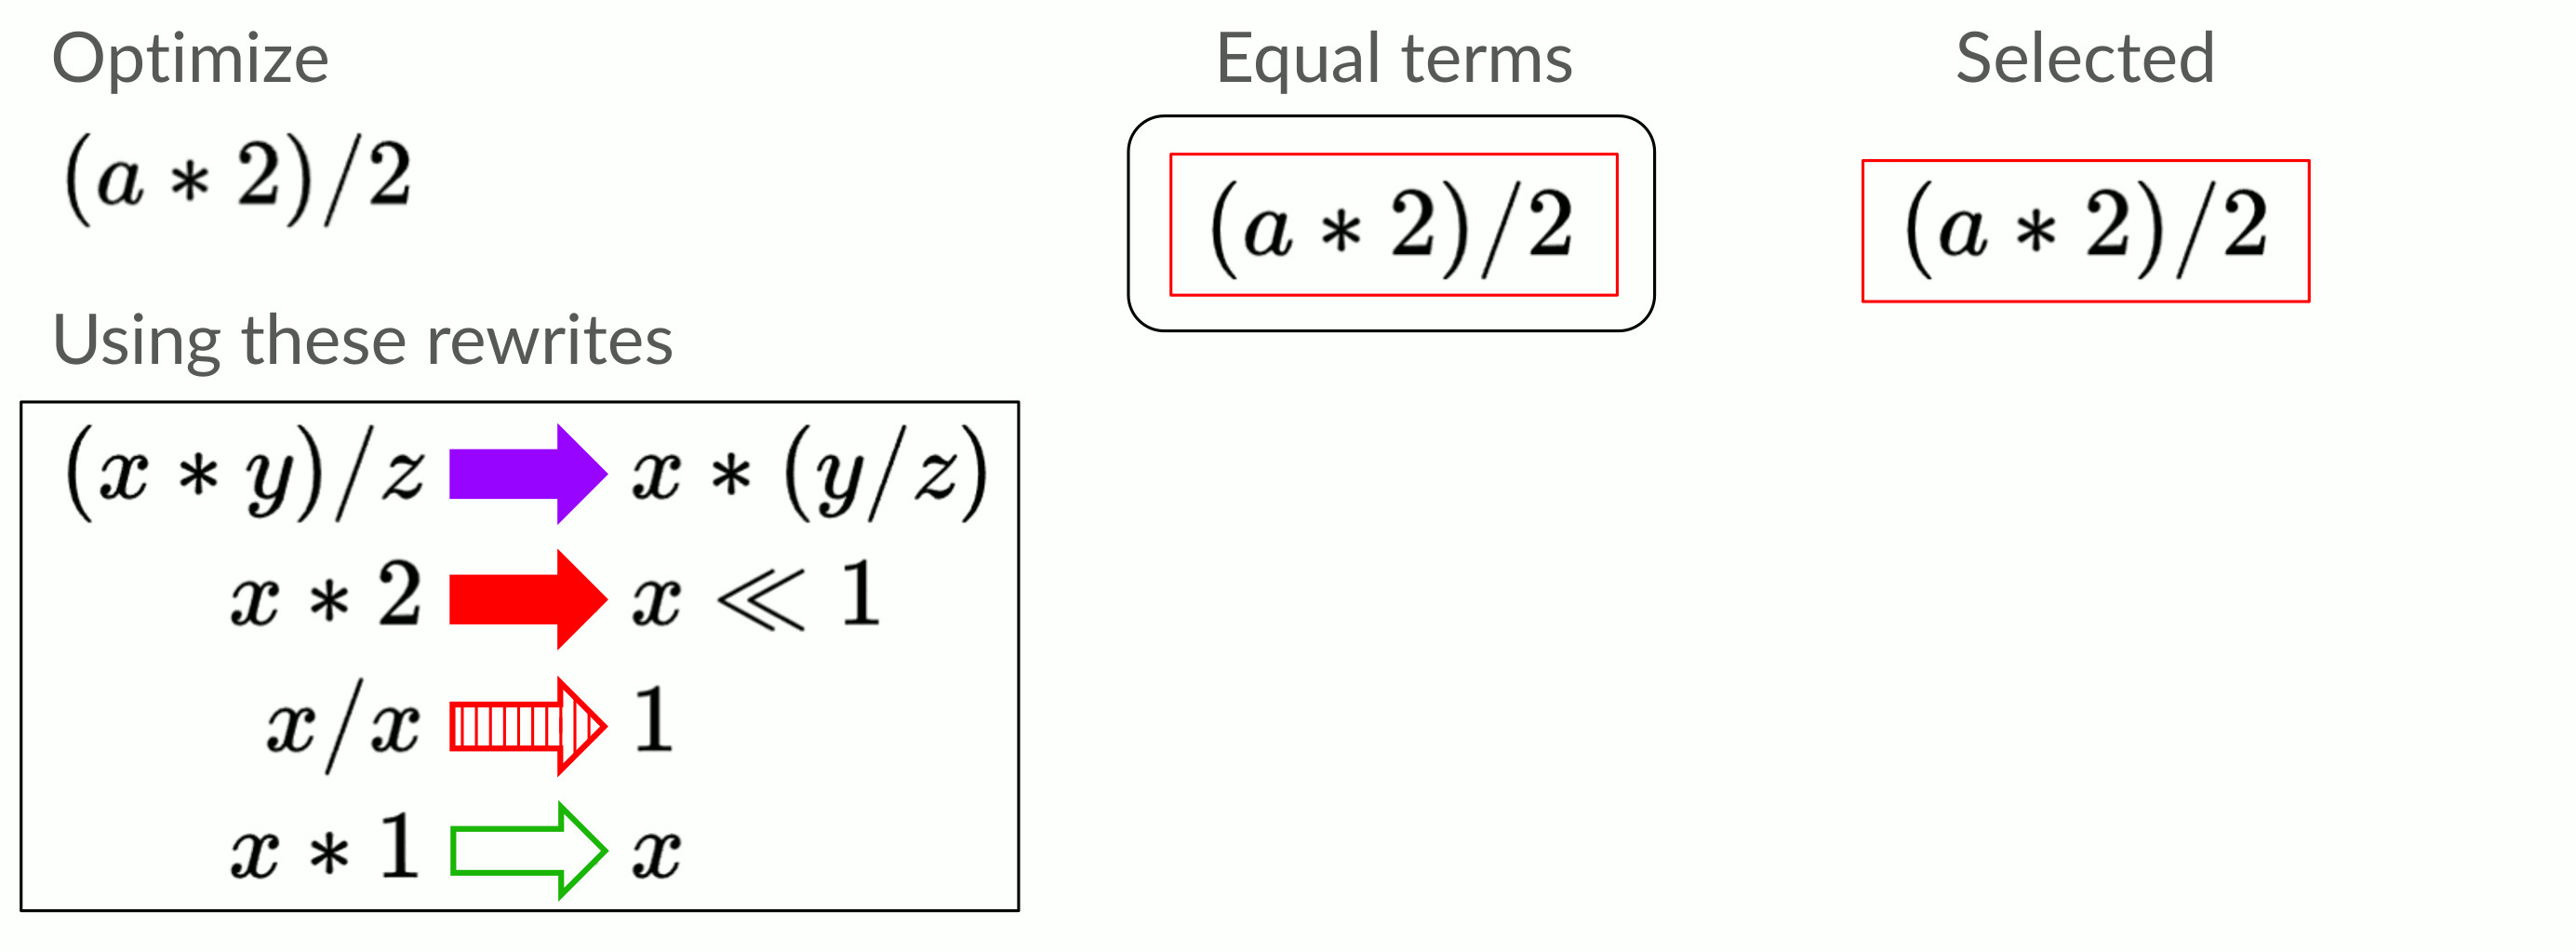
\includegraphics[width=13cm, height=5cm]{misc/egraphs_images//naive/n-1.jpg}
   }
   \only<3>
    {
        \centering
        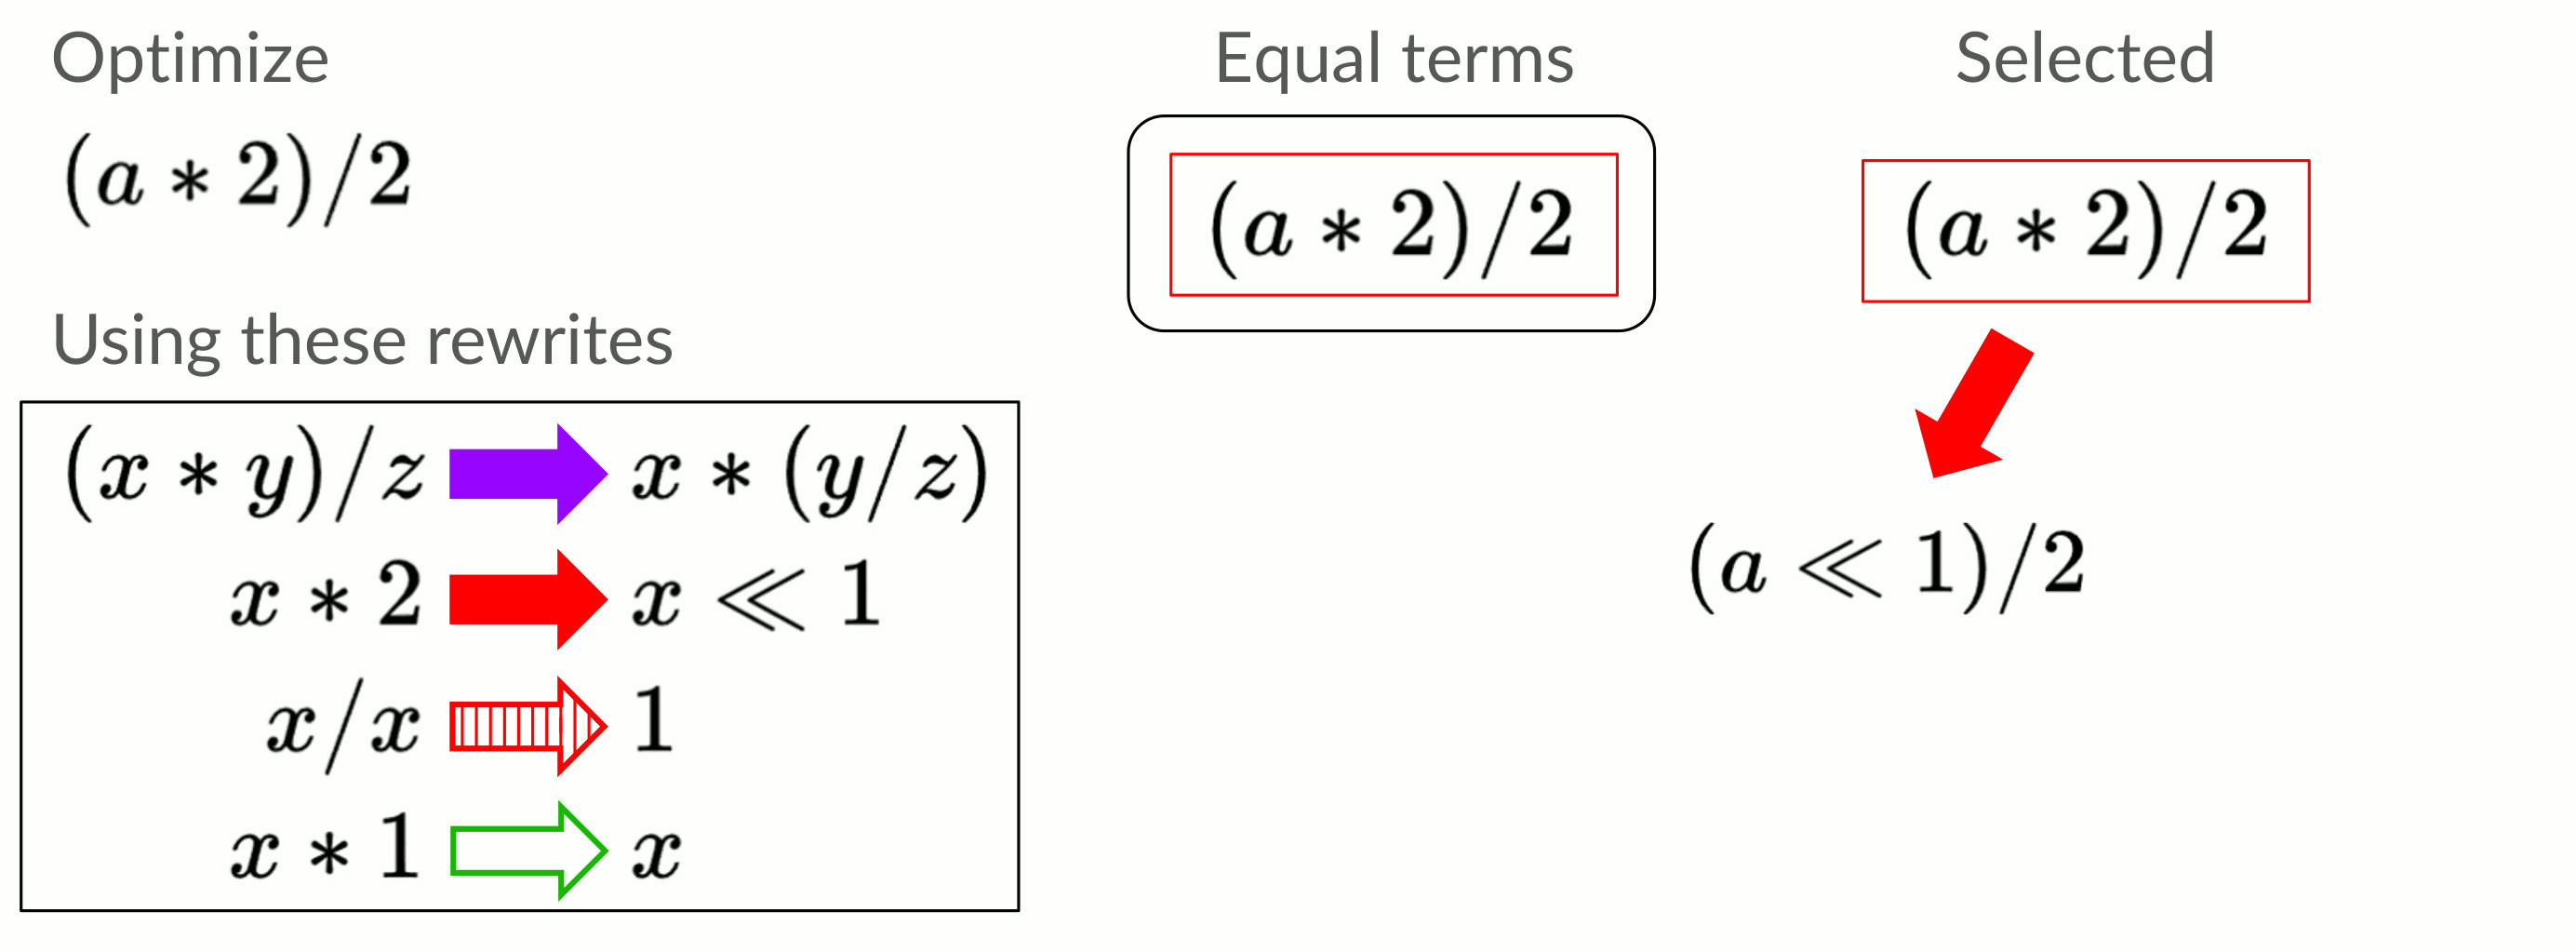
\includegraphics[width=13cm, height=5cm]{misc/egraphs_images/naive/n-2.jpg}
   }
   \only<4>
    {
        \centering
        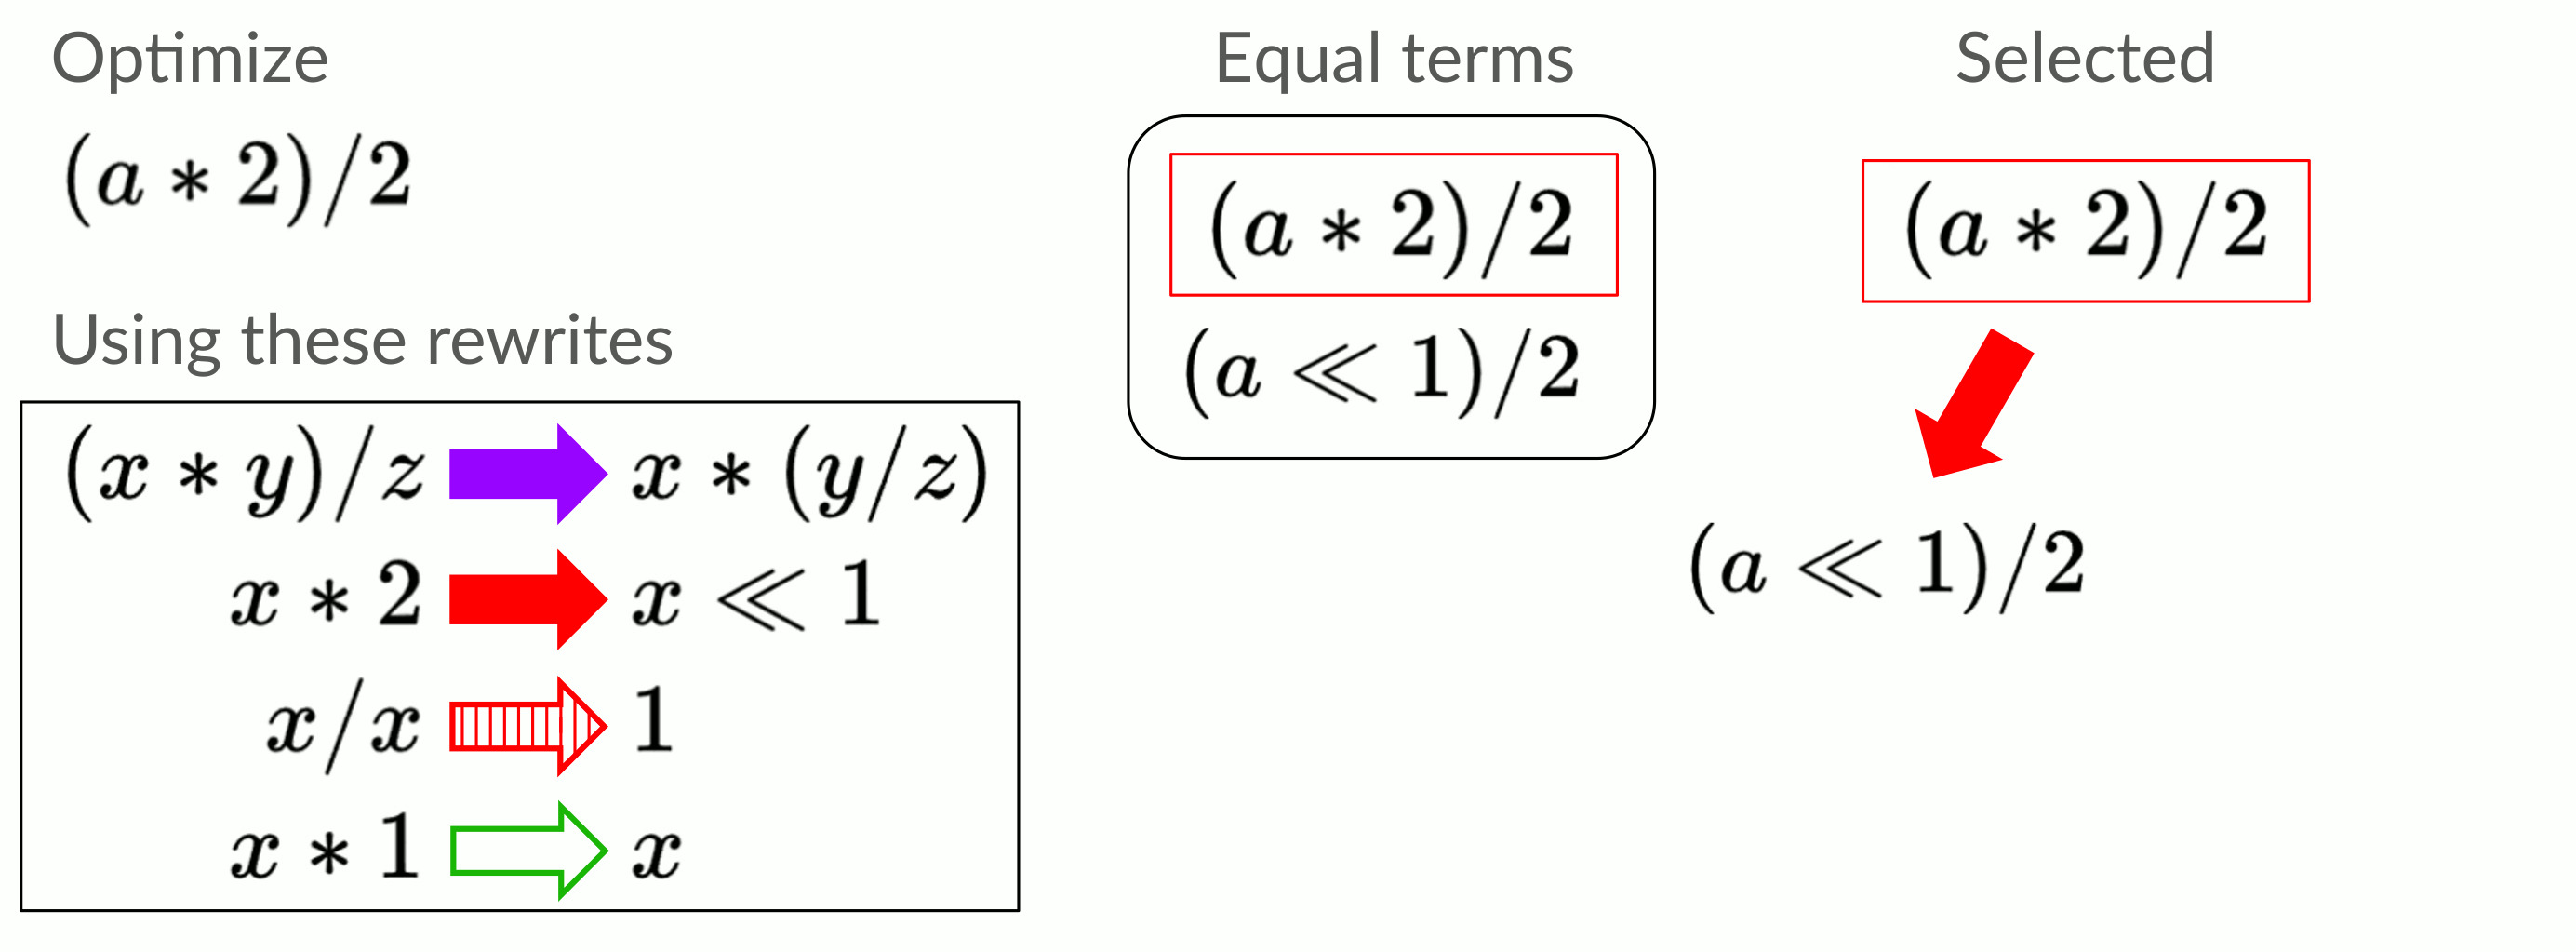
\includegraphics[width=13cm, height=5cm]{misc/egraphs_images/naive/n-3.jpg}
   }
    \only<5>
    {
        \centering
        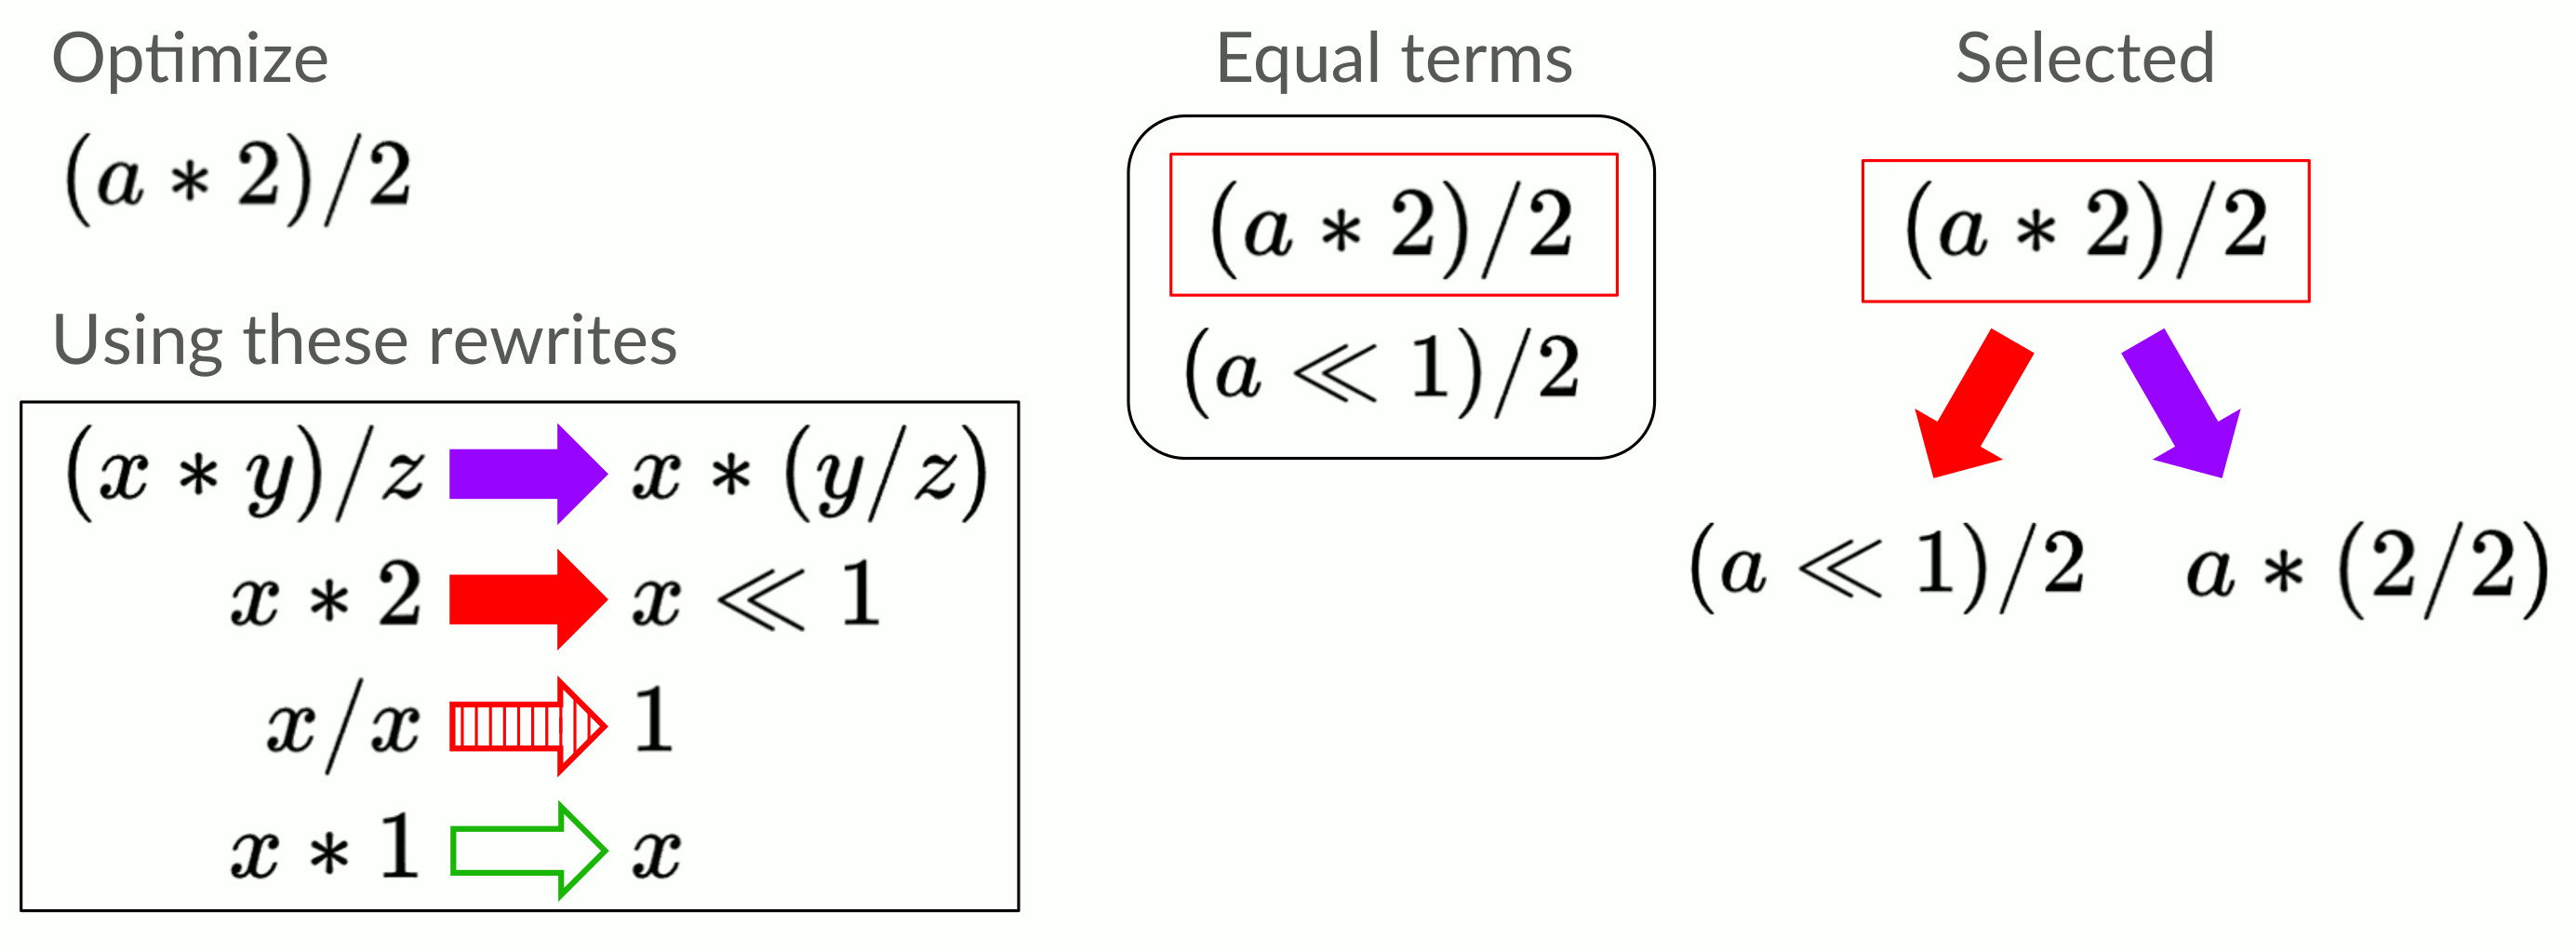
\includegraphics[width=13cm, height=5cm]{misc/egraphs_images/naive/n-4.jpg}
   }
    \only<6>
    {
        \centering
        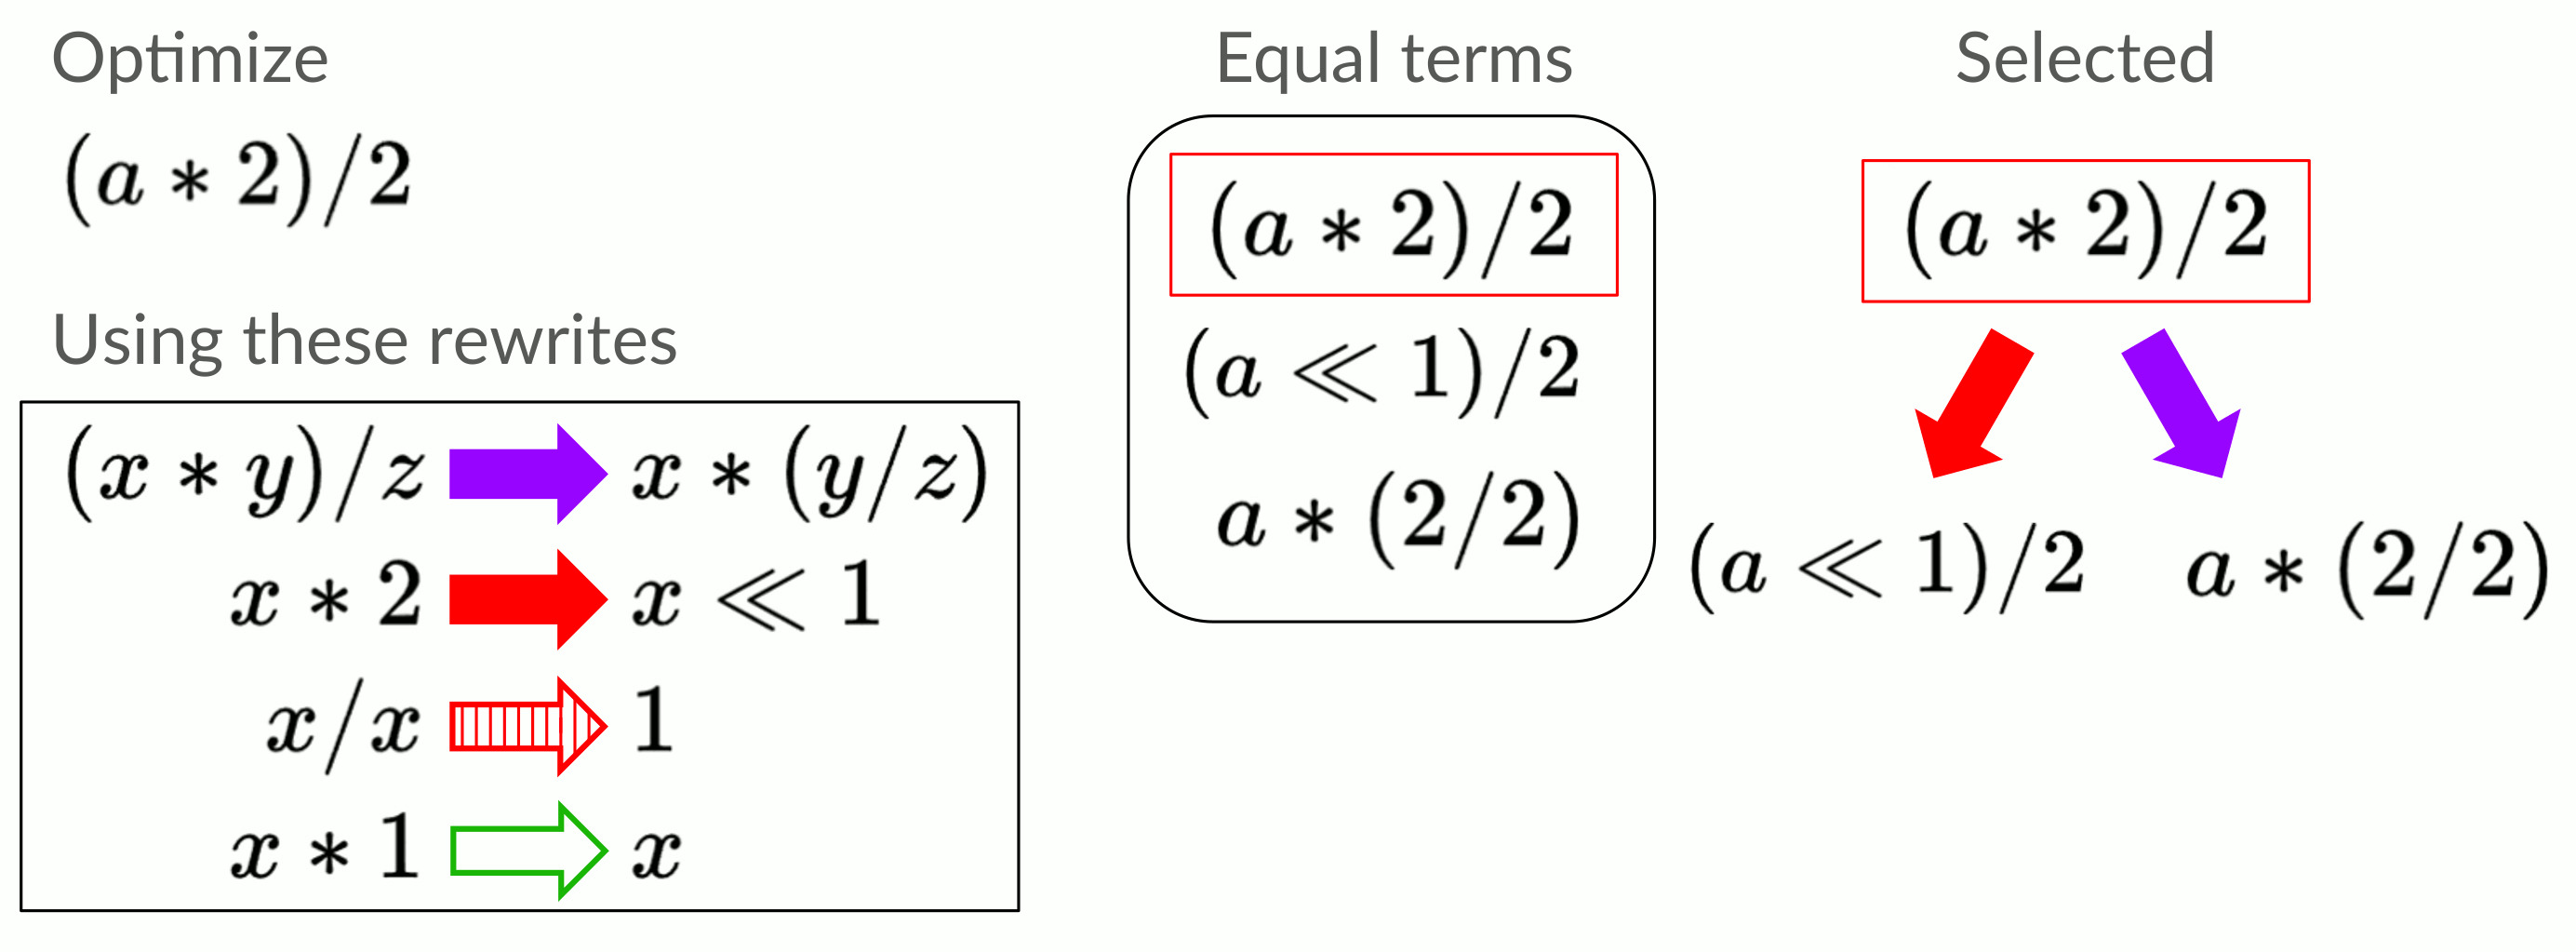
\includegraphics[width=13cm, height=5cm]{misc/egraphs_images/naive/n-5.jpg}
   }
   \only<7>
    {
        \centering
        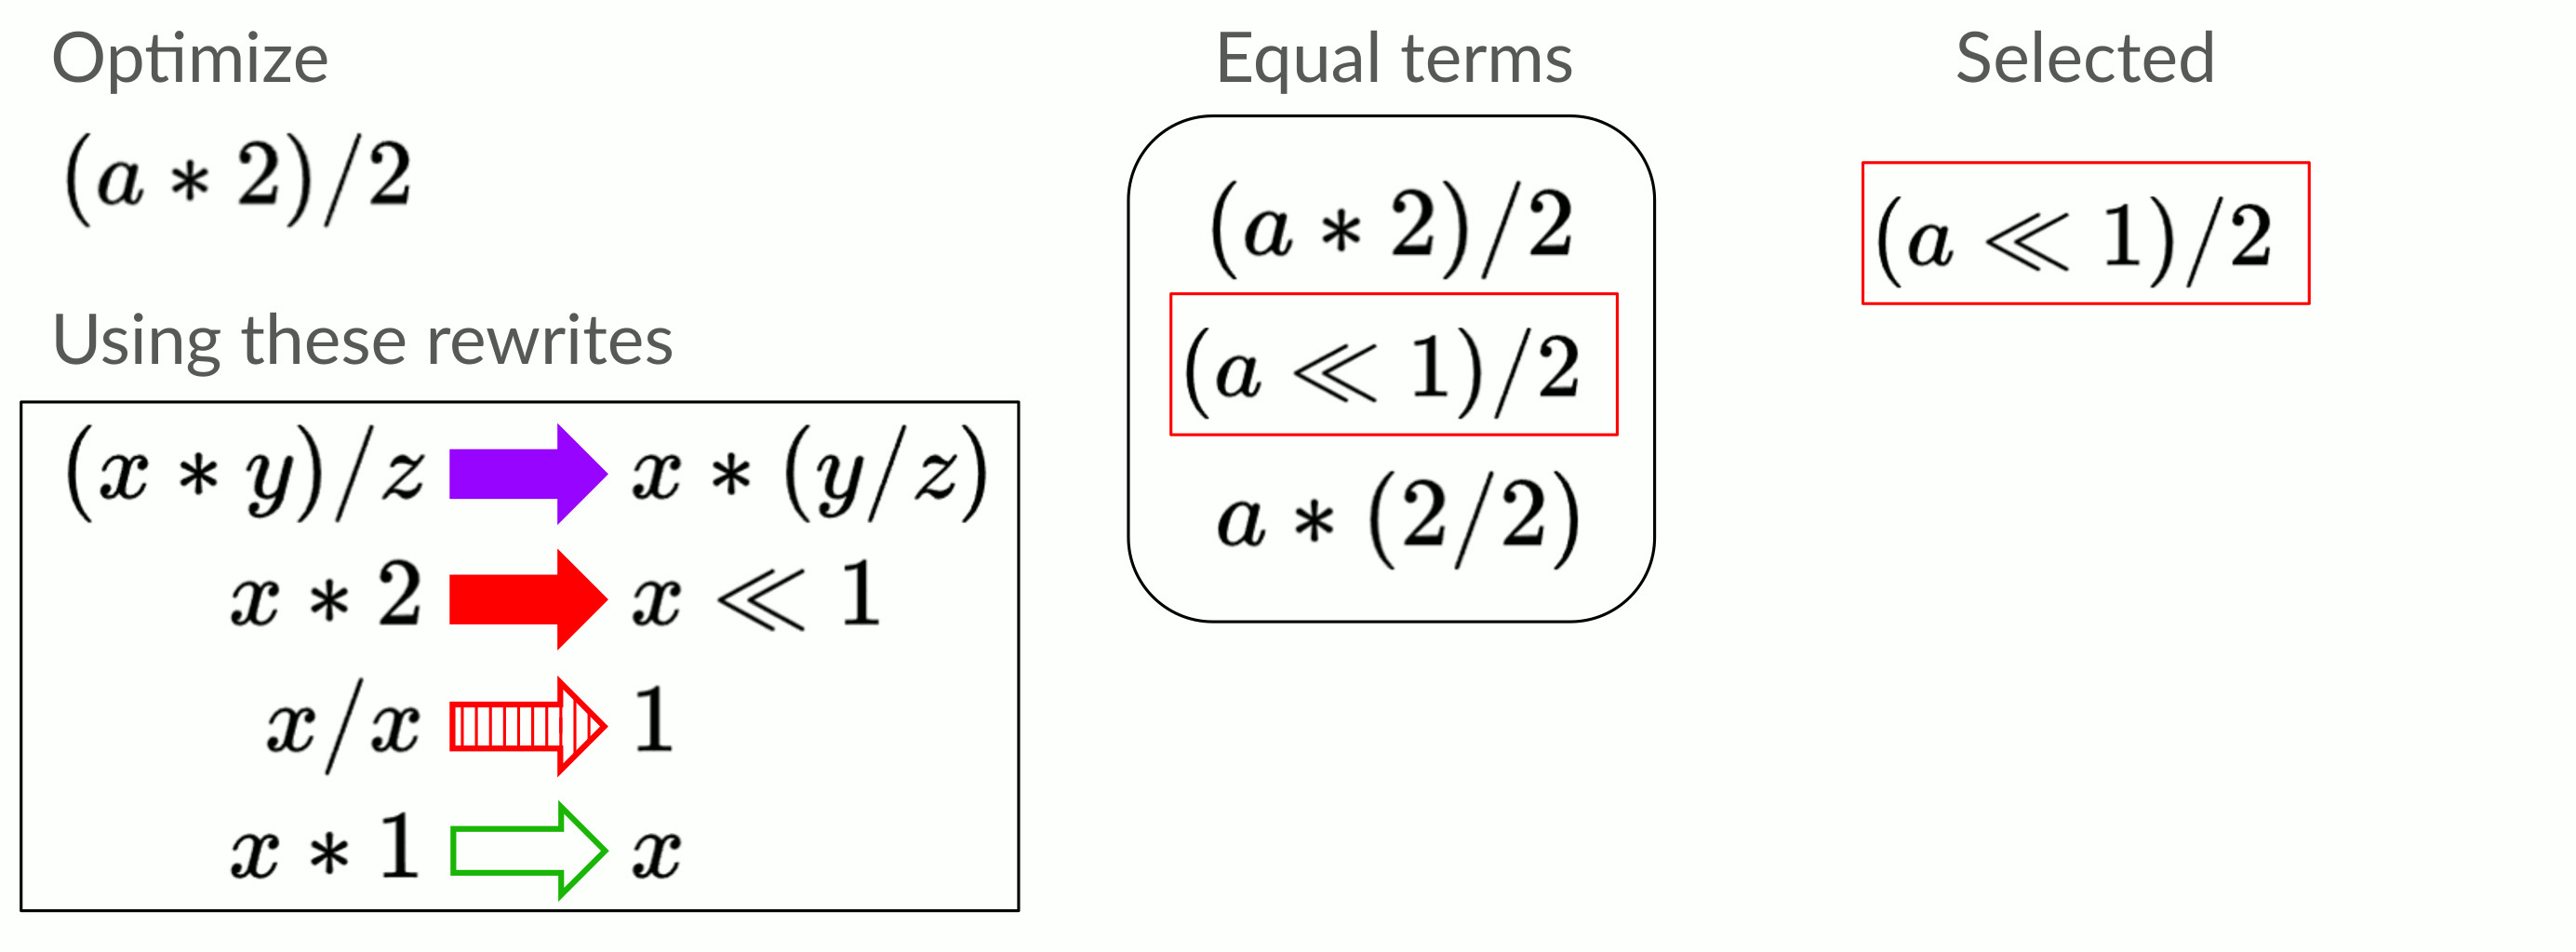
\includegraphics[width=13cm, height=5cm]{misc/egraphs_images/naive/n-6.jpg}
   }
   \only<8>
    {
        \centering
        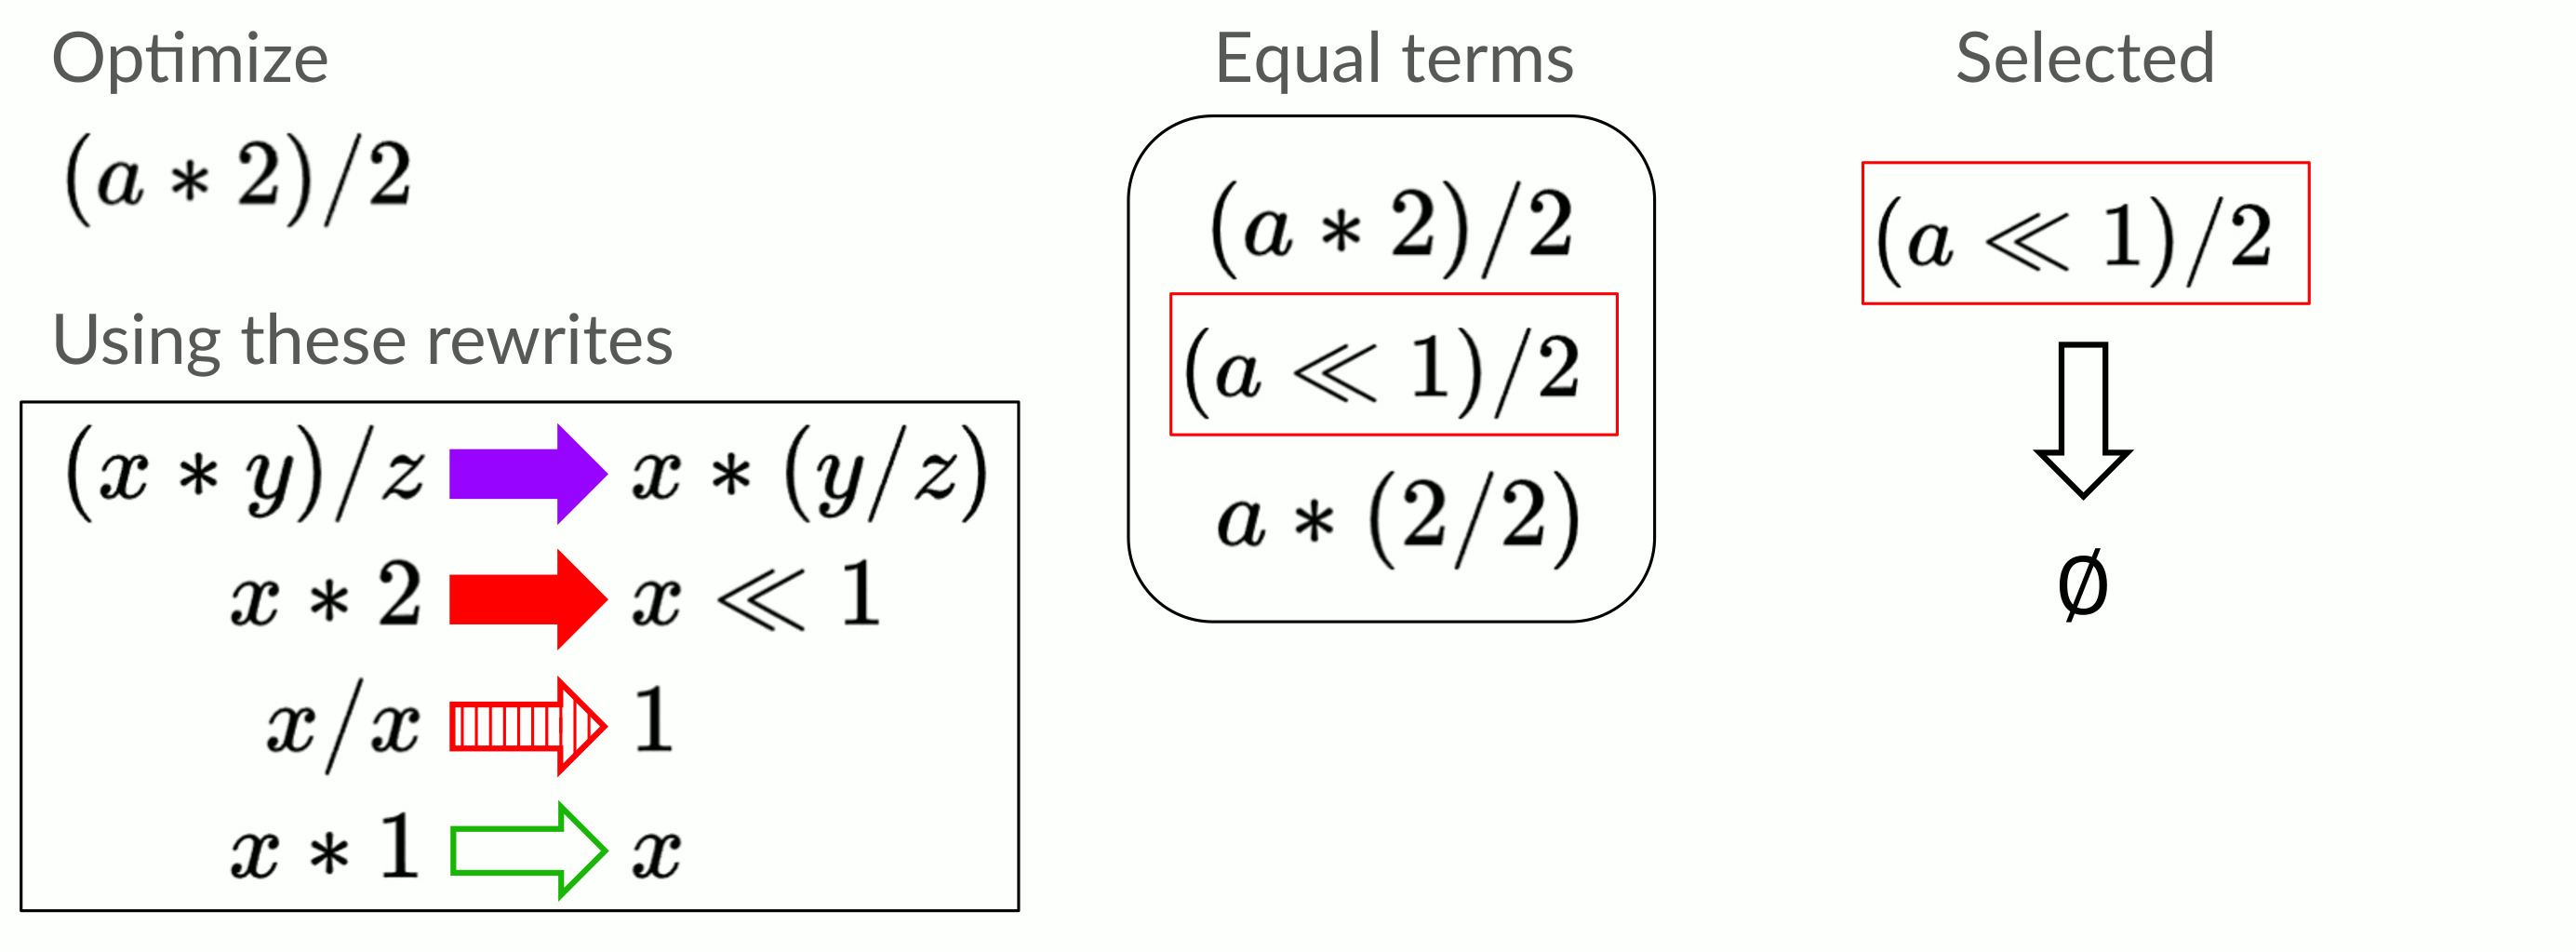
\includegraphics[width=13cm, height=5cm]{misc/egraphs_images/naive/n-7.jpg}
   }
   \only<9>
    {
        \centering
        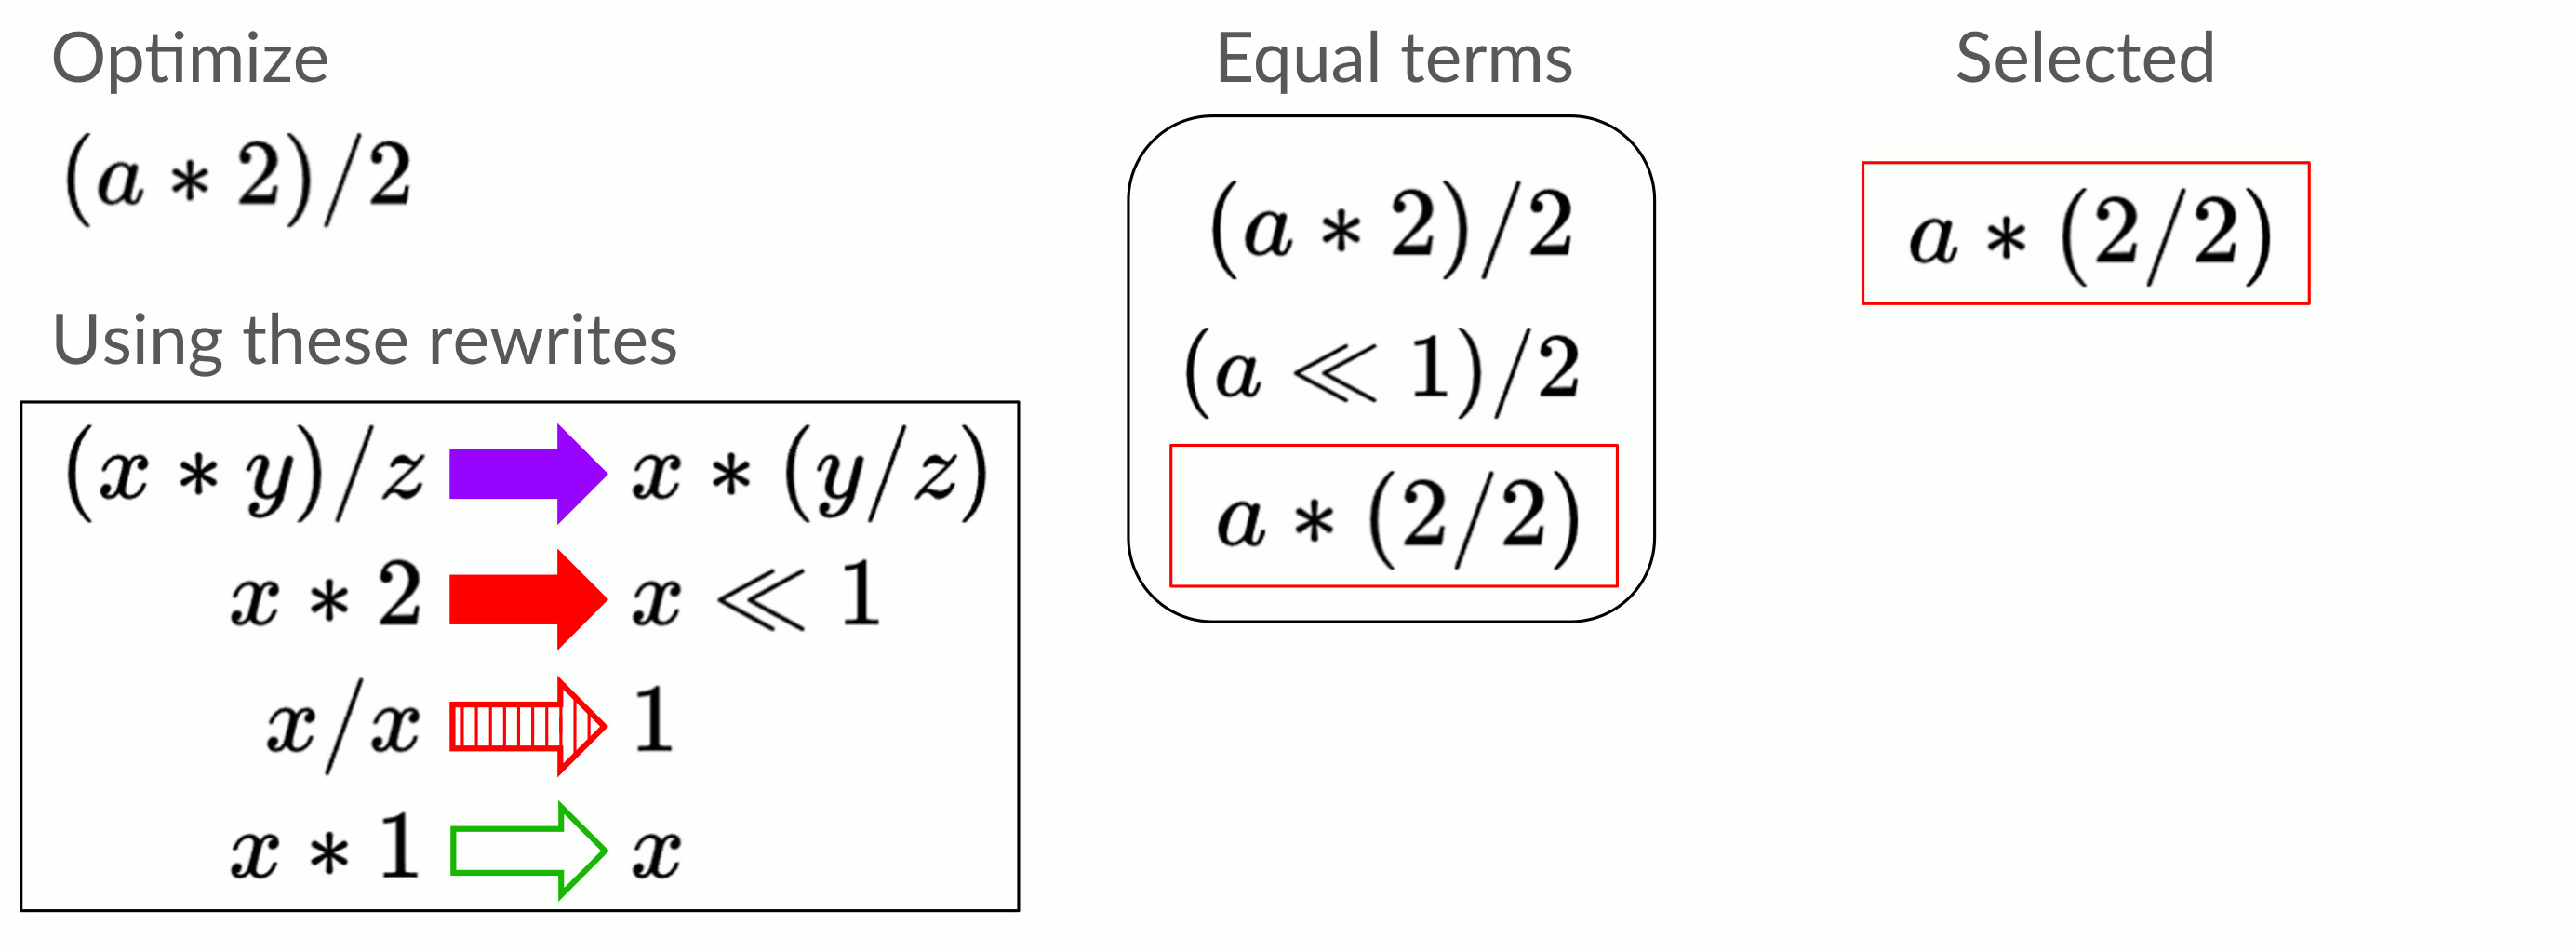
\includegraphics[width=13cm, height=5cm]{misc/egraphs_images/naive/n-8.jpg}
   }
   \only<10>
    {
        \centering
        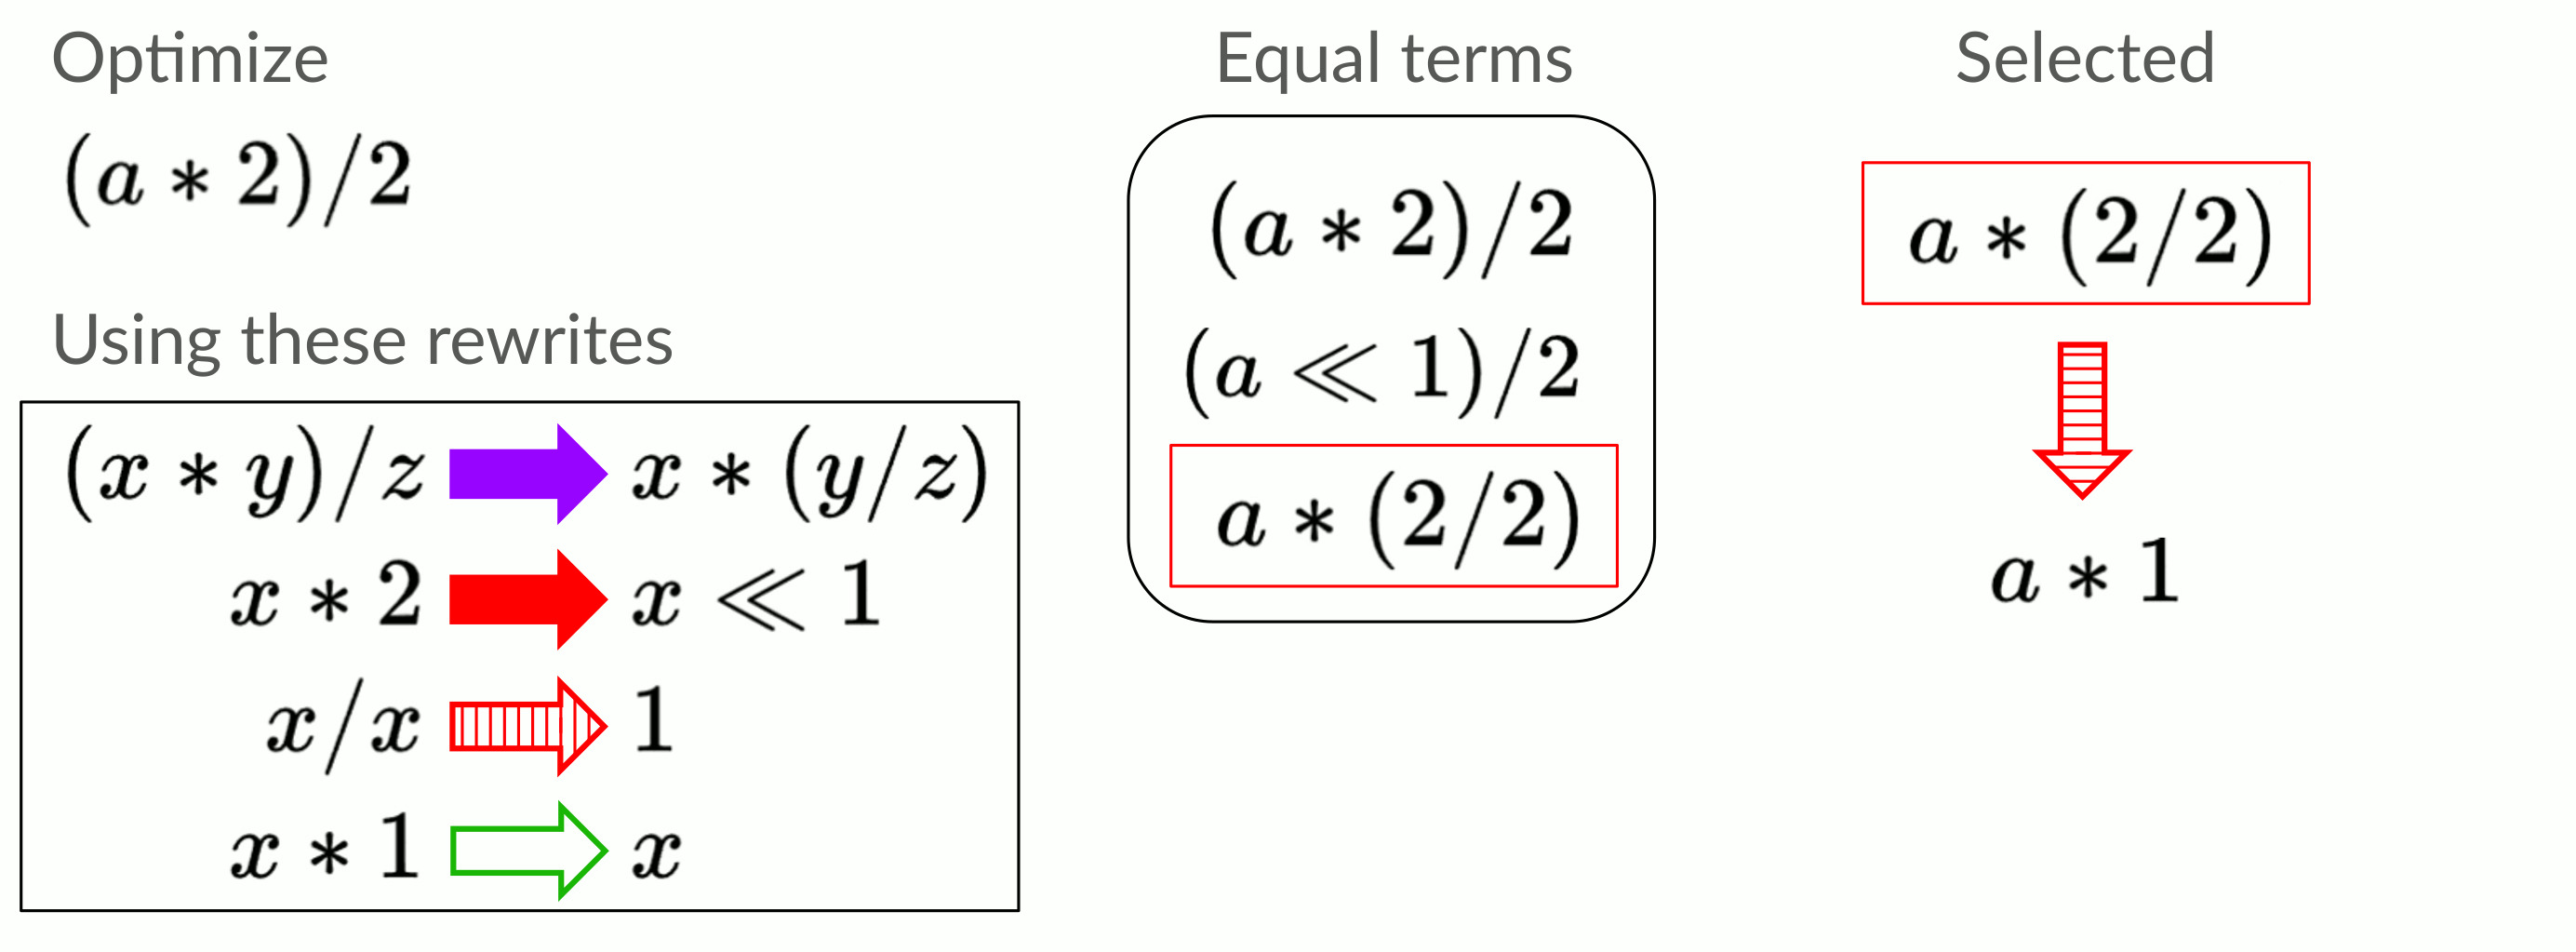
\includegraphics[width=13cm, height=5cm]{misc/egraphs_images/naive/n-9.jpg}
   }
   \only<11>
    {
        \centering
        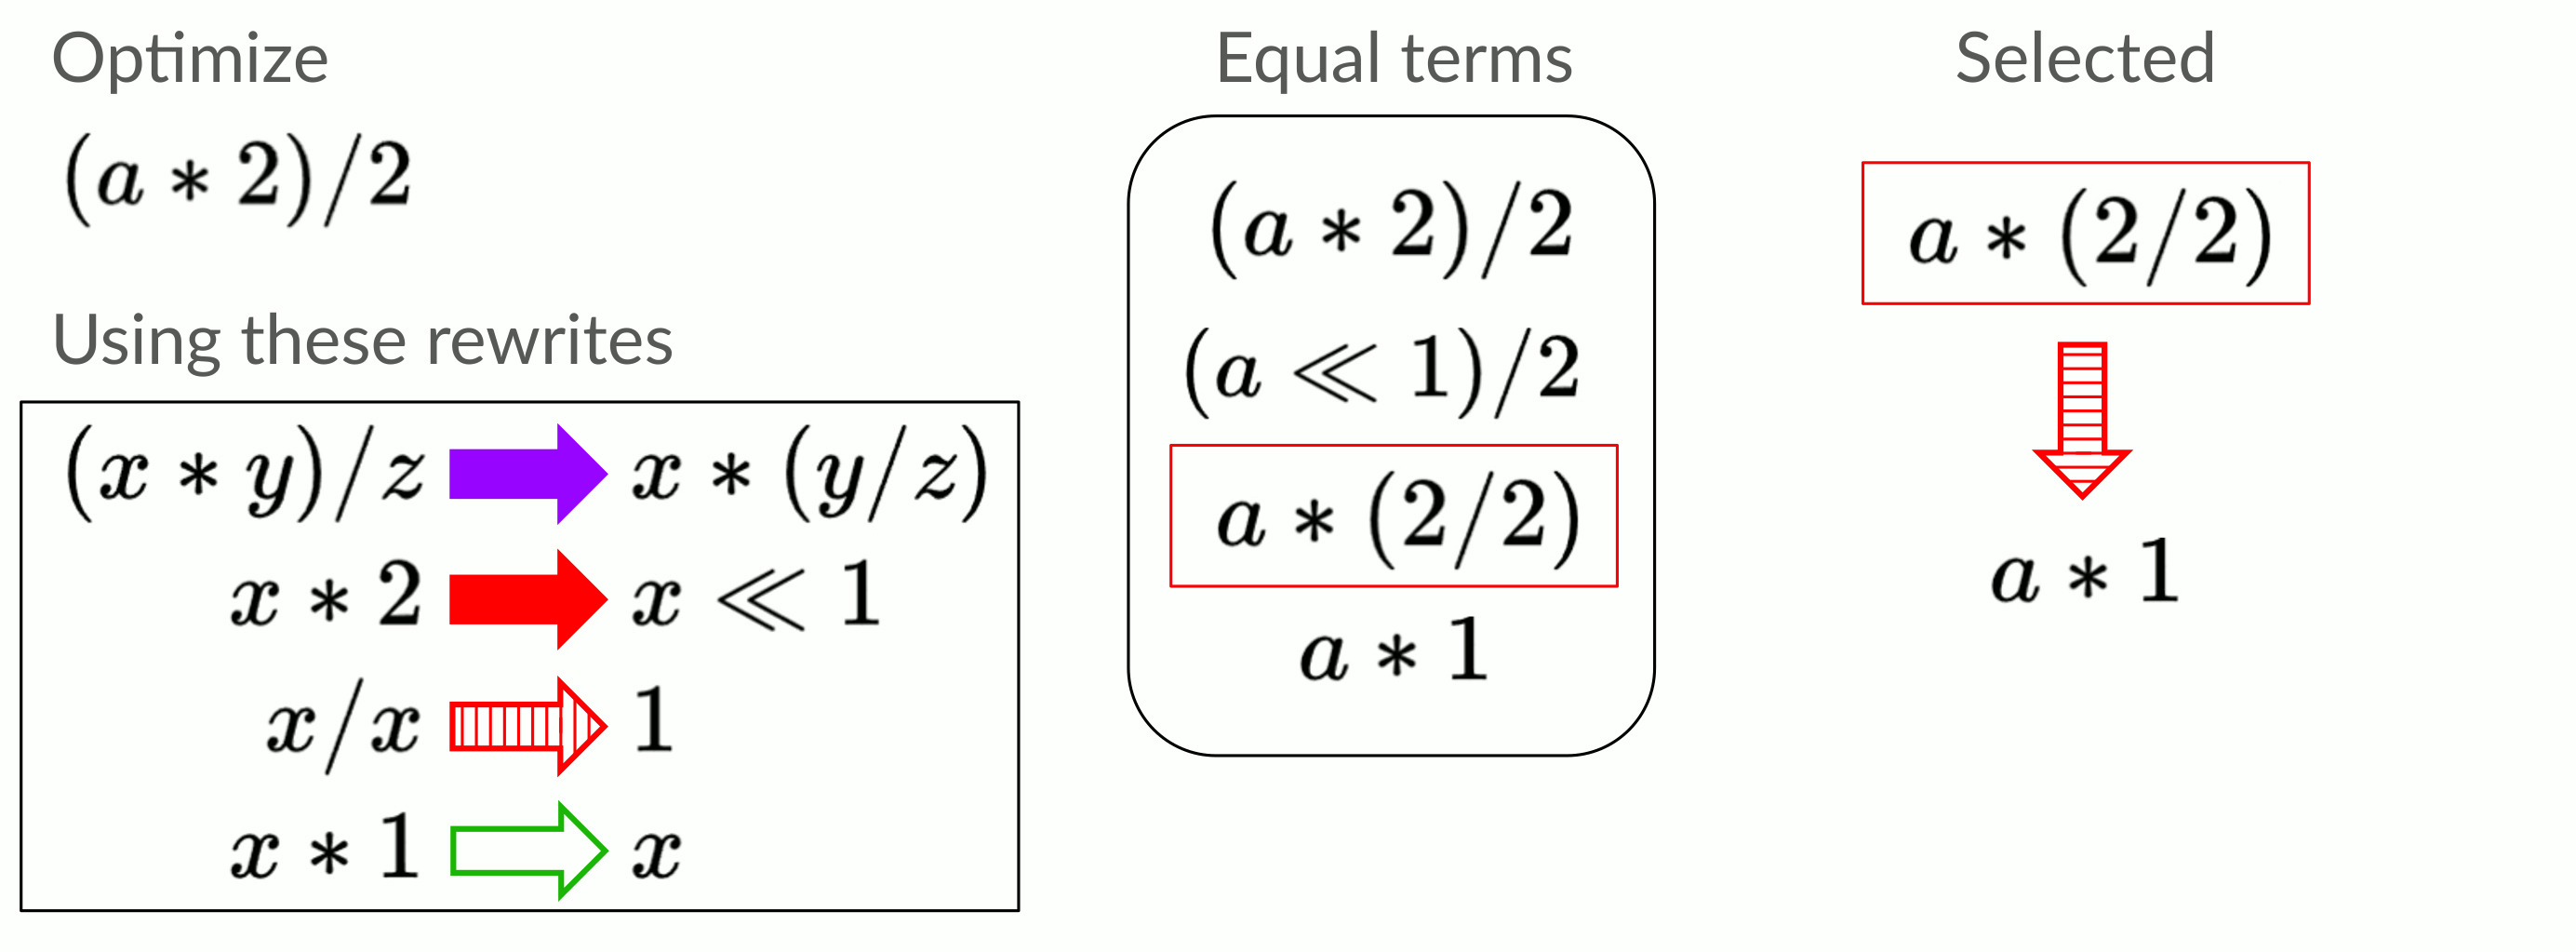
\includegraphics[width=13cm, height=5cm]{misc/egraphs_images/naive/n-10.jpg}
   }
   \only<12>
    {
        \centering
        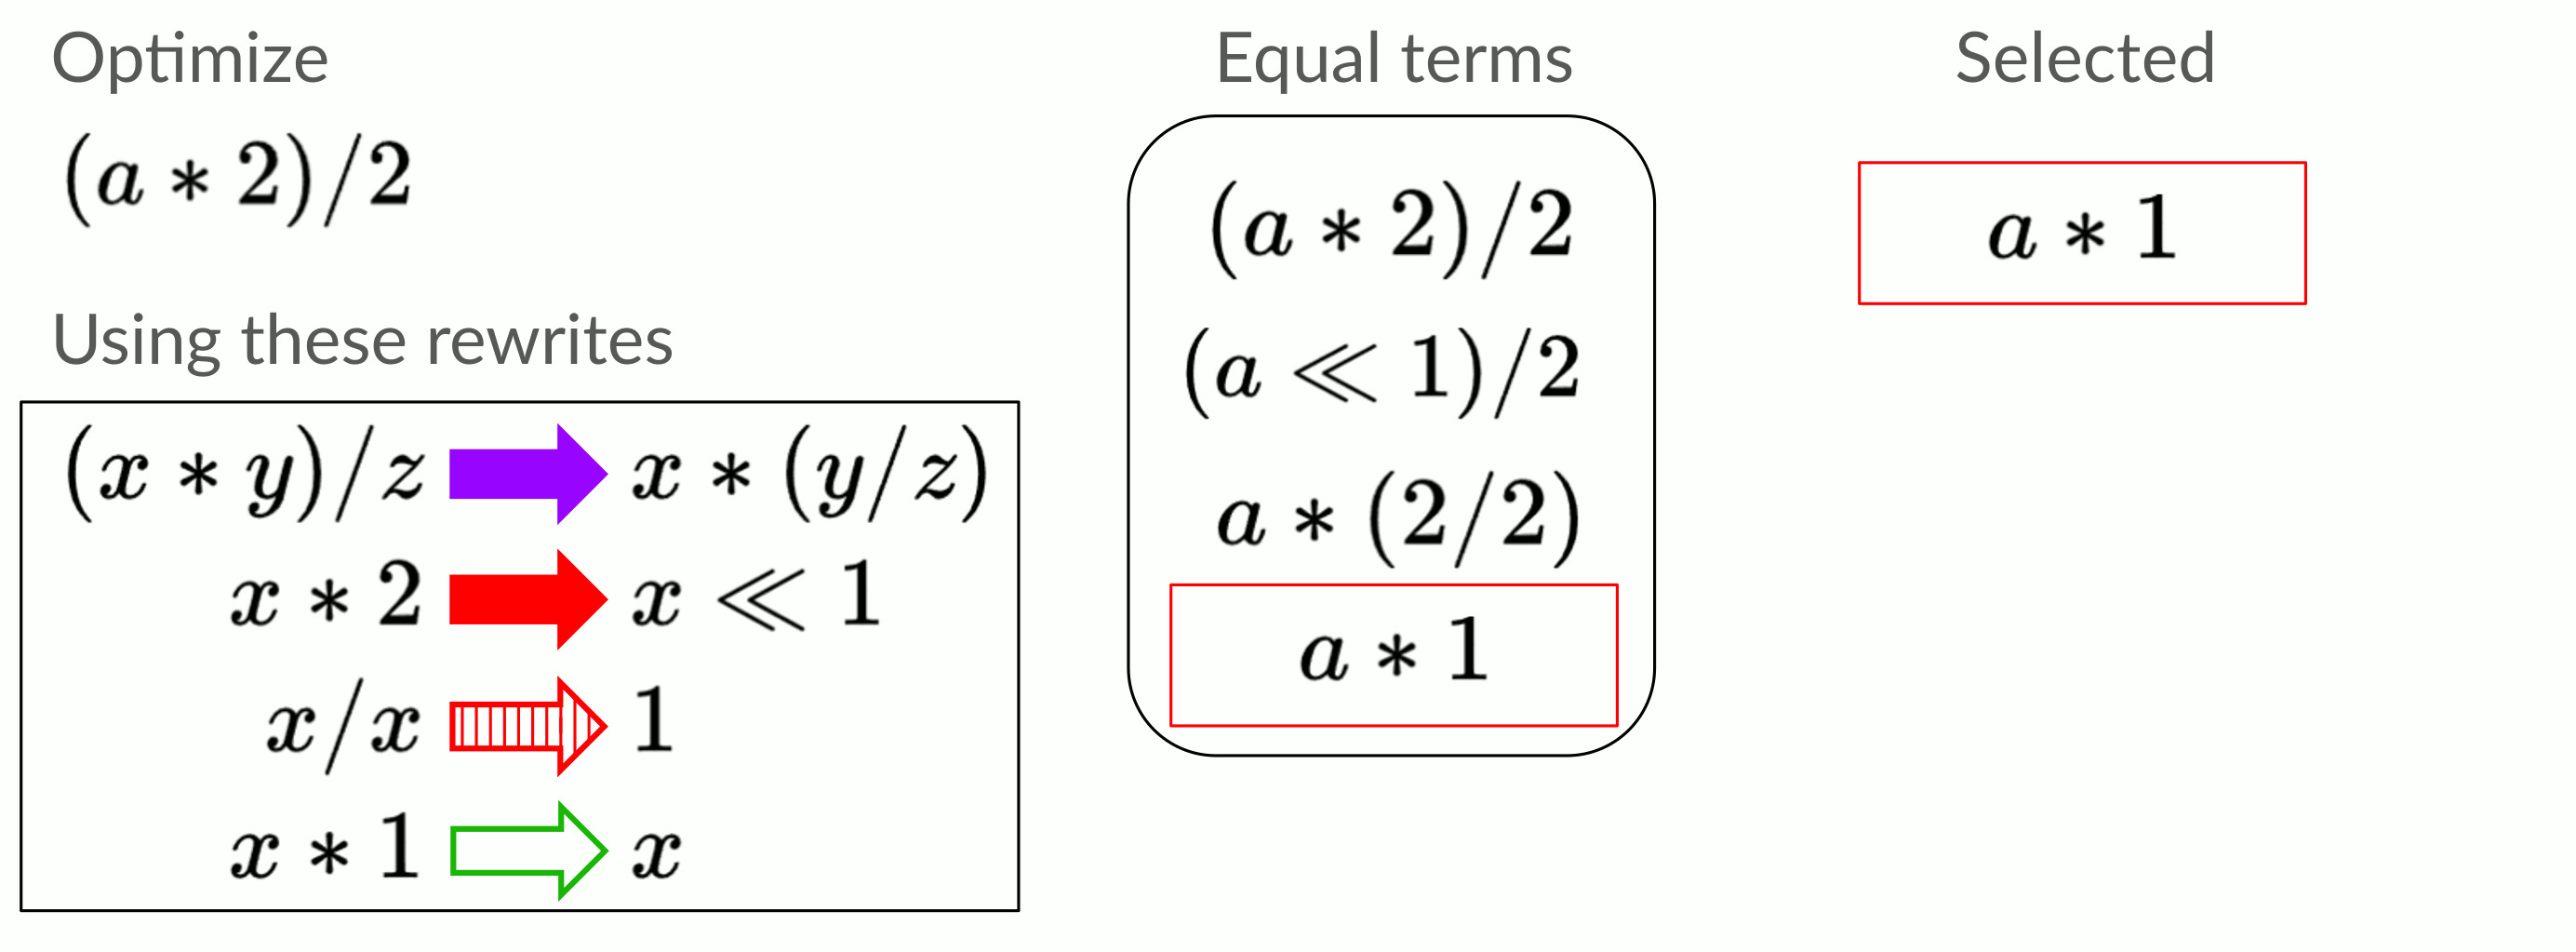
\includegraphics[width=13cm, height=5cm]{misc/egraphs_images/naive/n-11.jpg}
   }
   \only<13>
    {
        \centering
        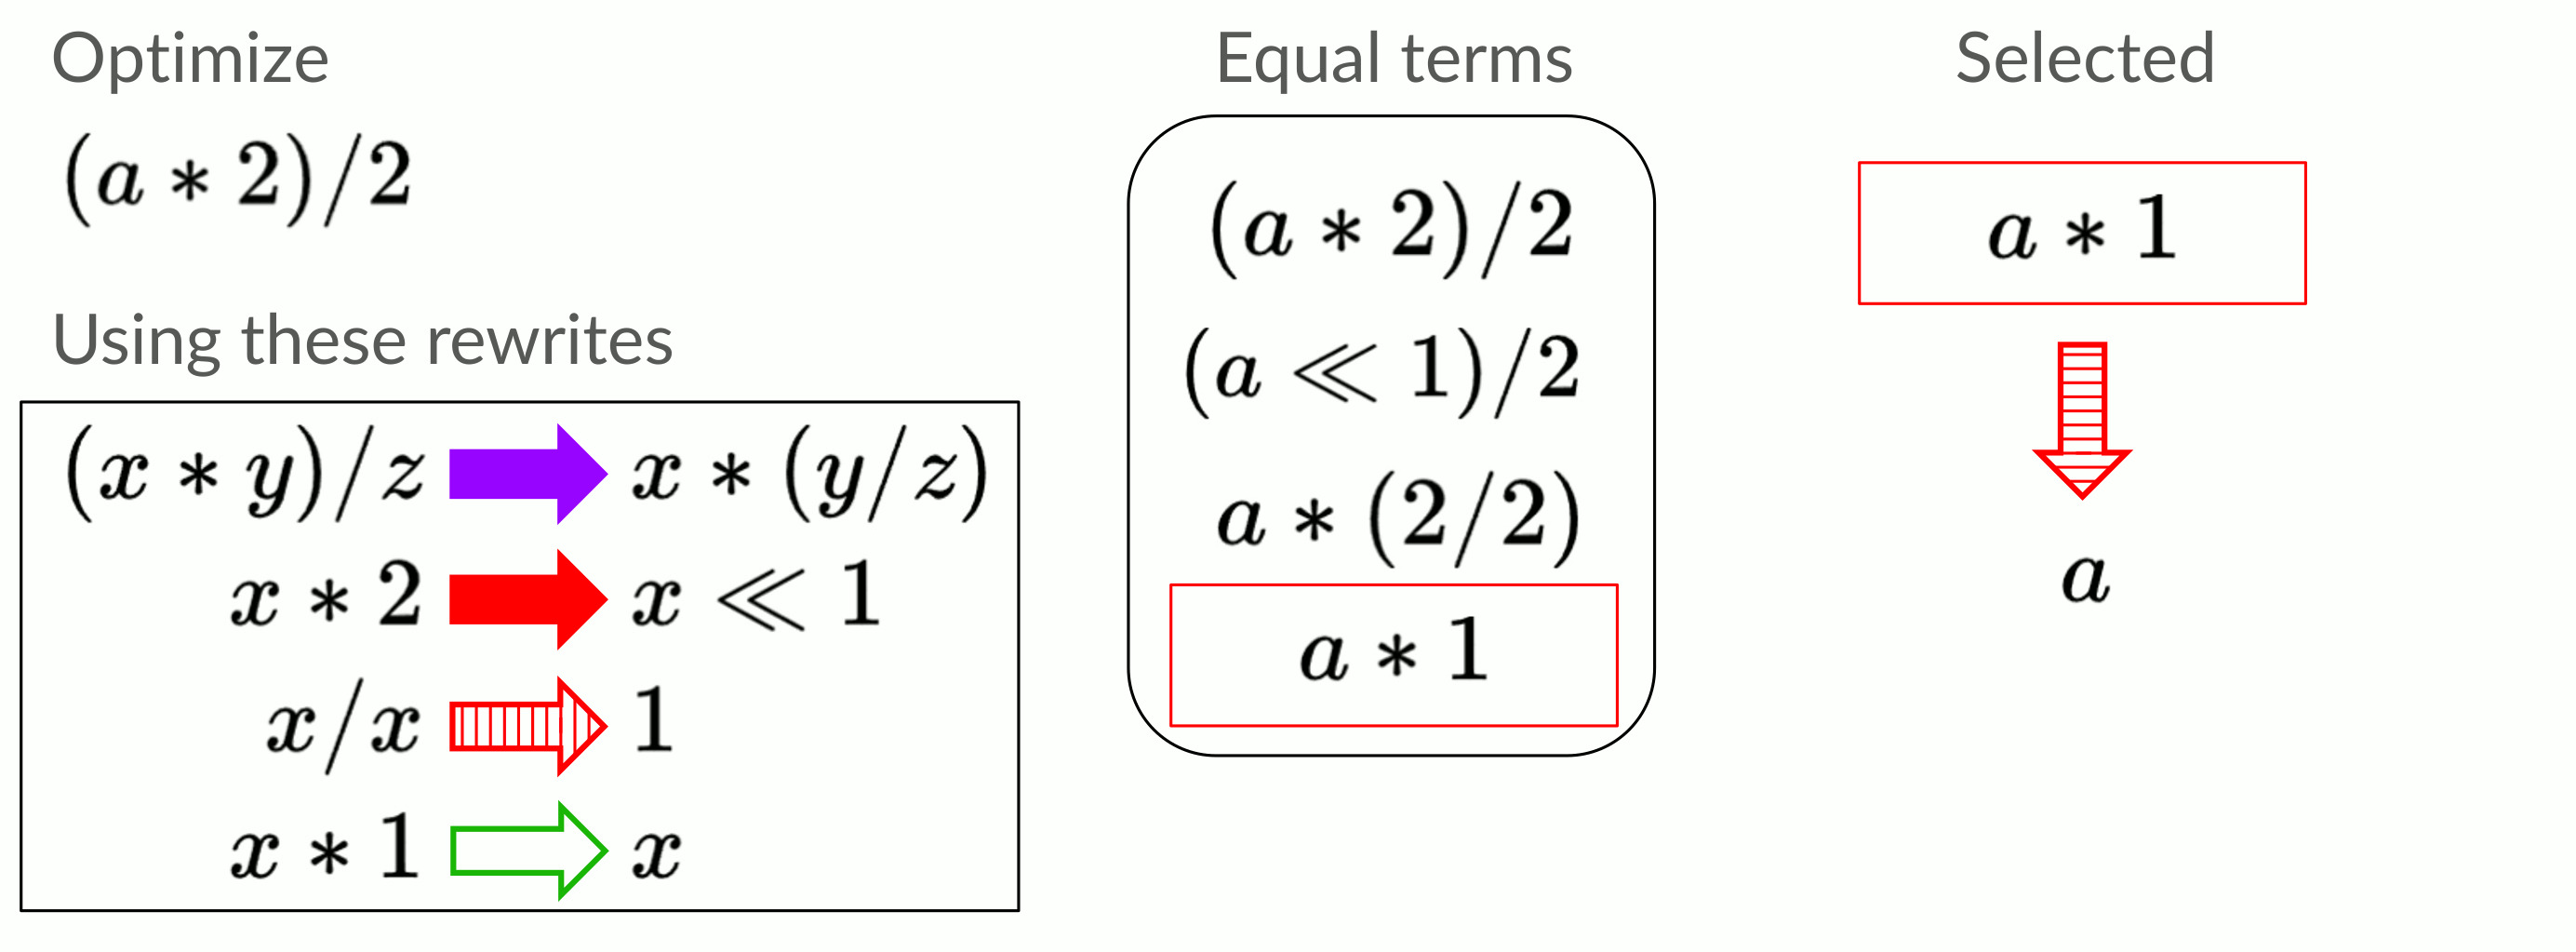
\includegraphics[width=13cm, height=5cm]{misc/egraphs_images/naive/n-12.jpg}
   }
   \only<14>
    {
        \centering
        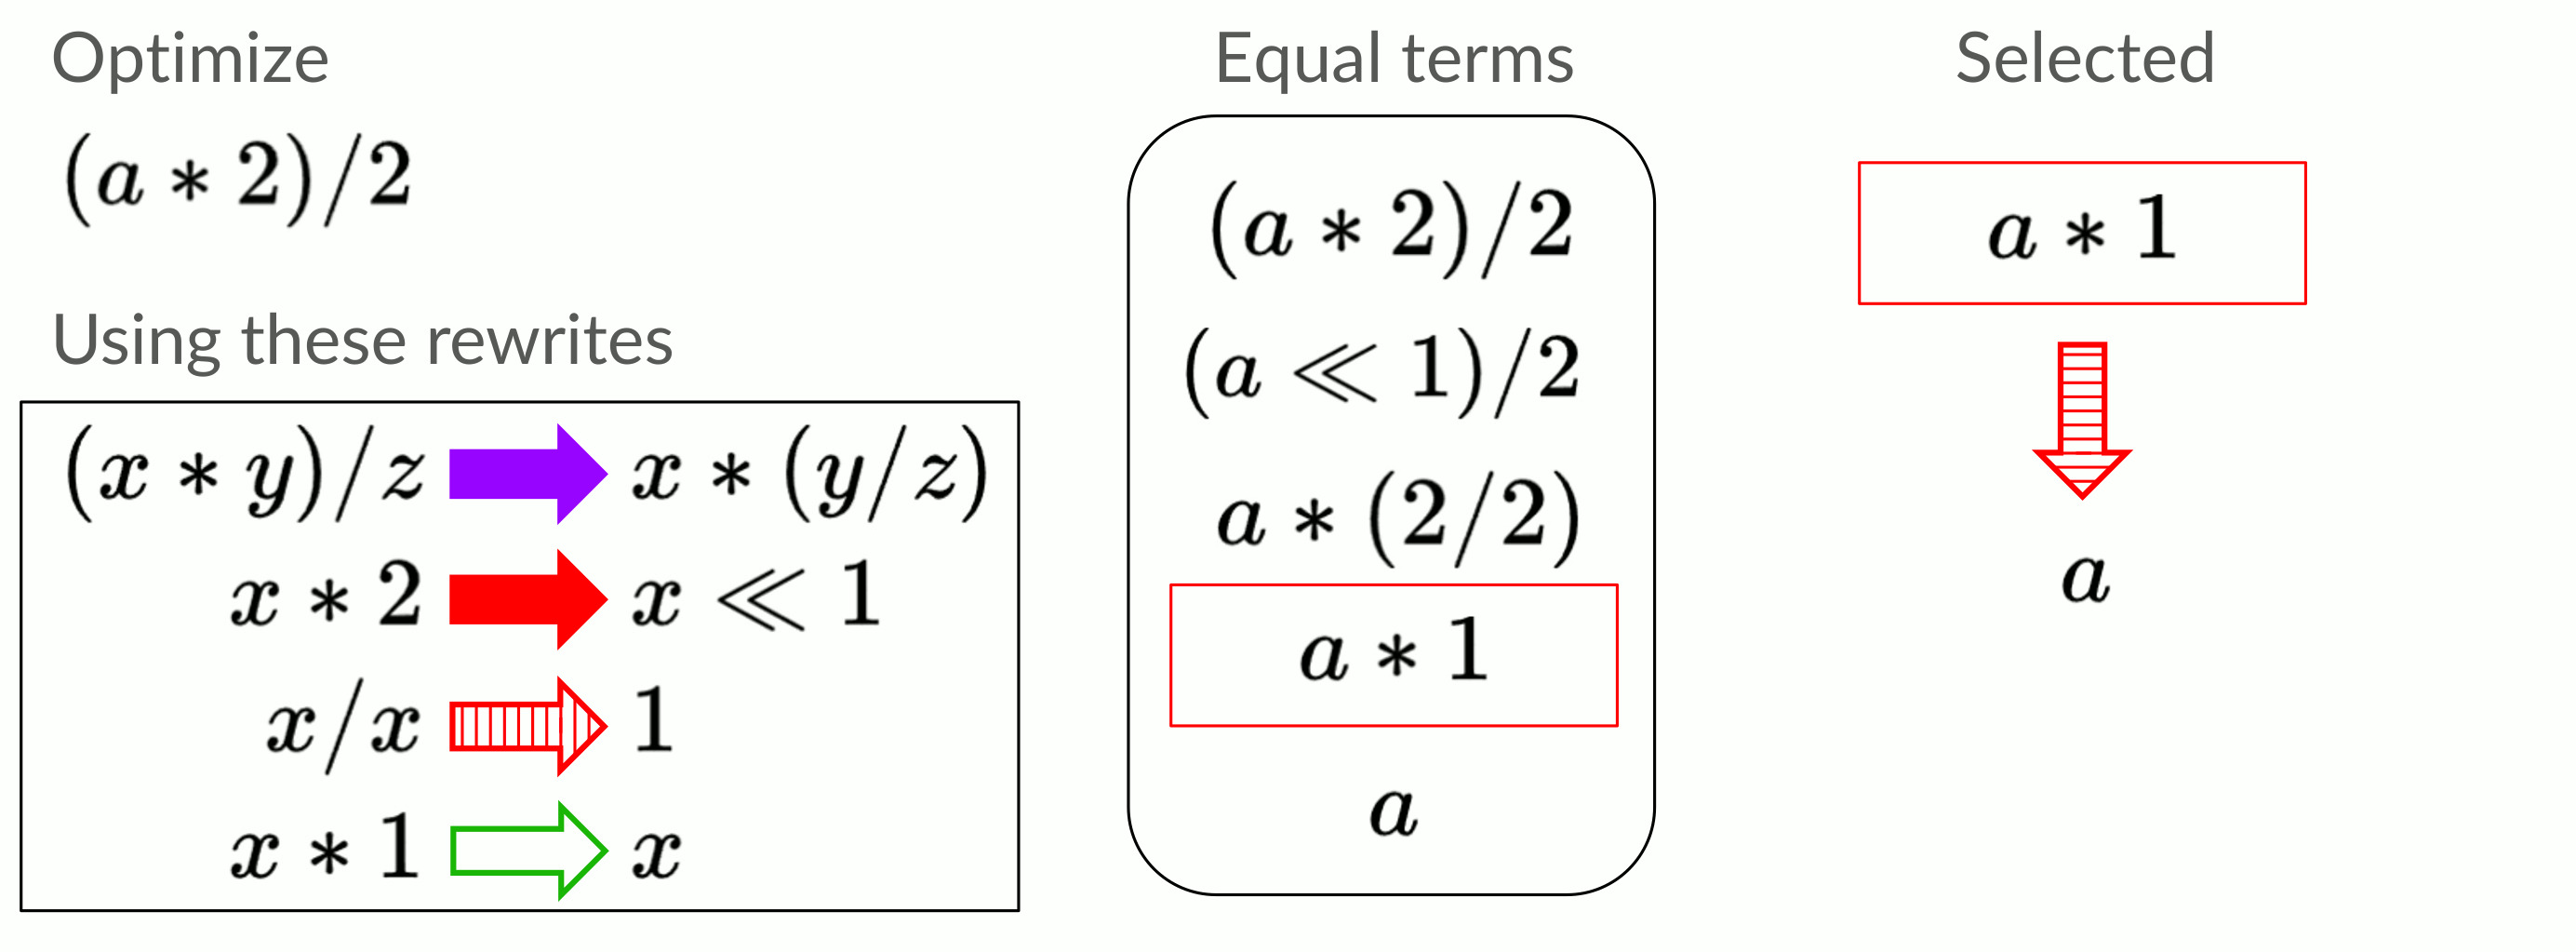
\includegraphics[width=13cm, height=5cm]{misc/egraphs_images/naive/n-13.jpg}
   }
   \only<15>
    {
        \centering
        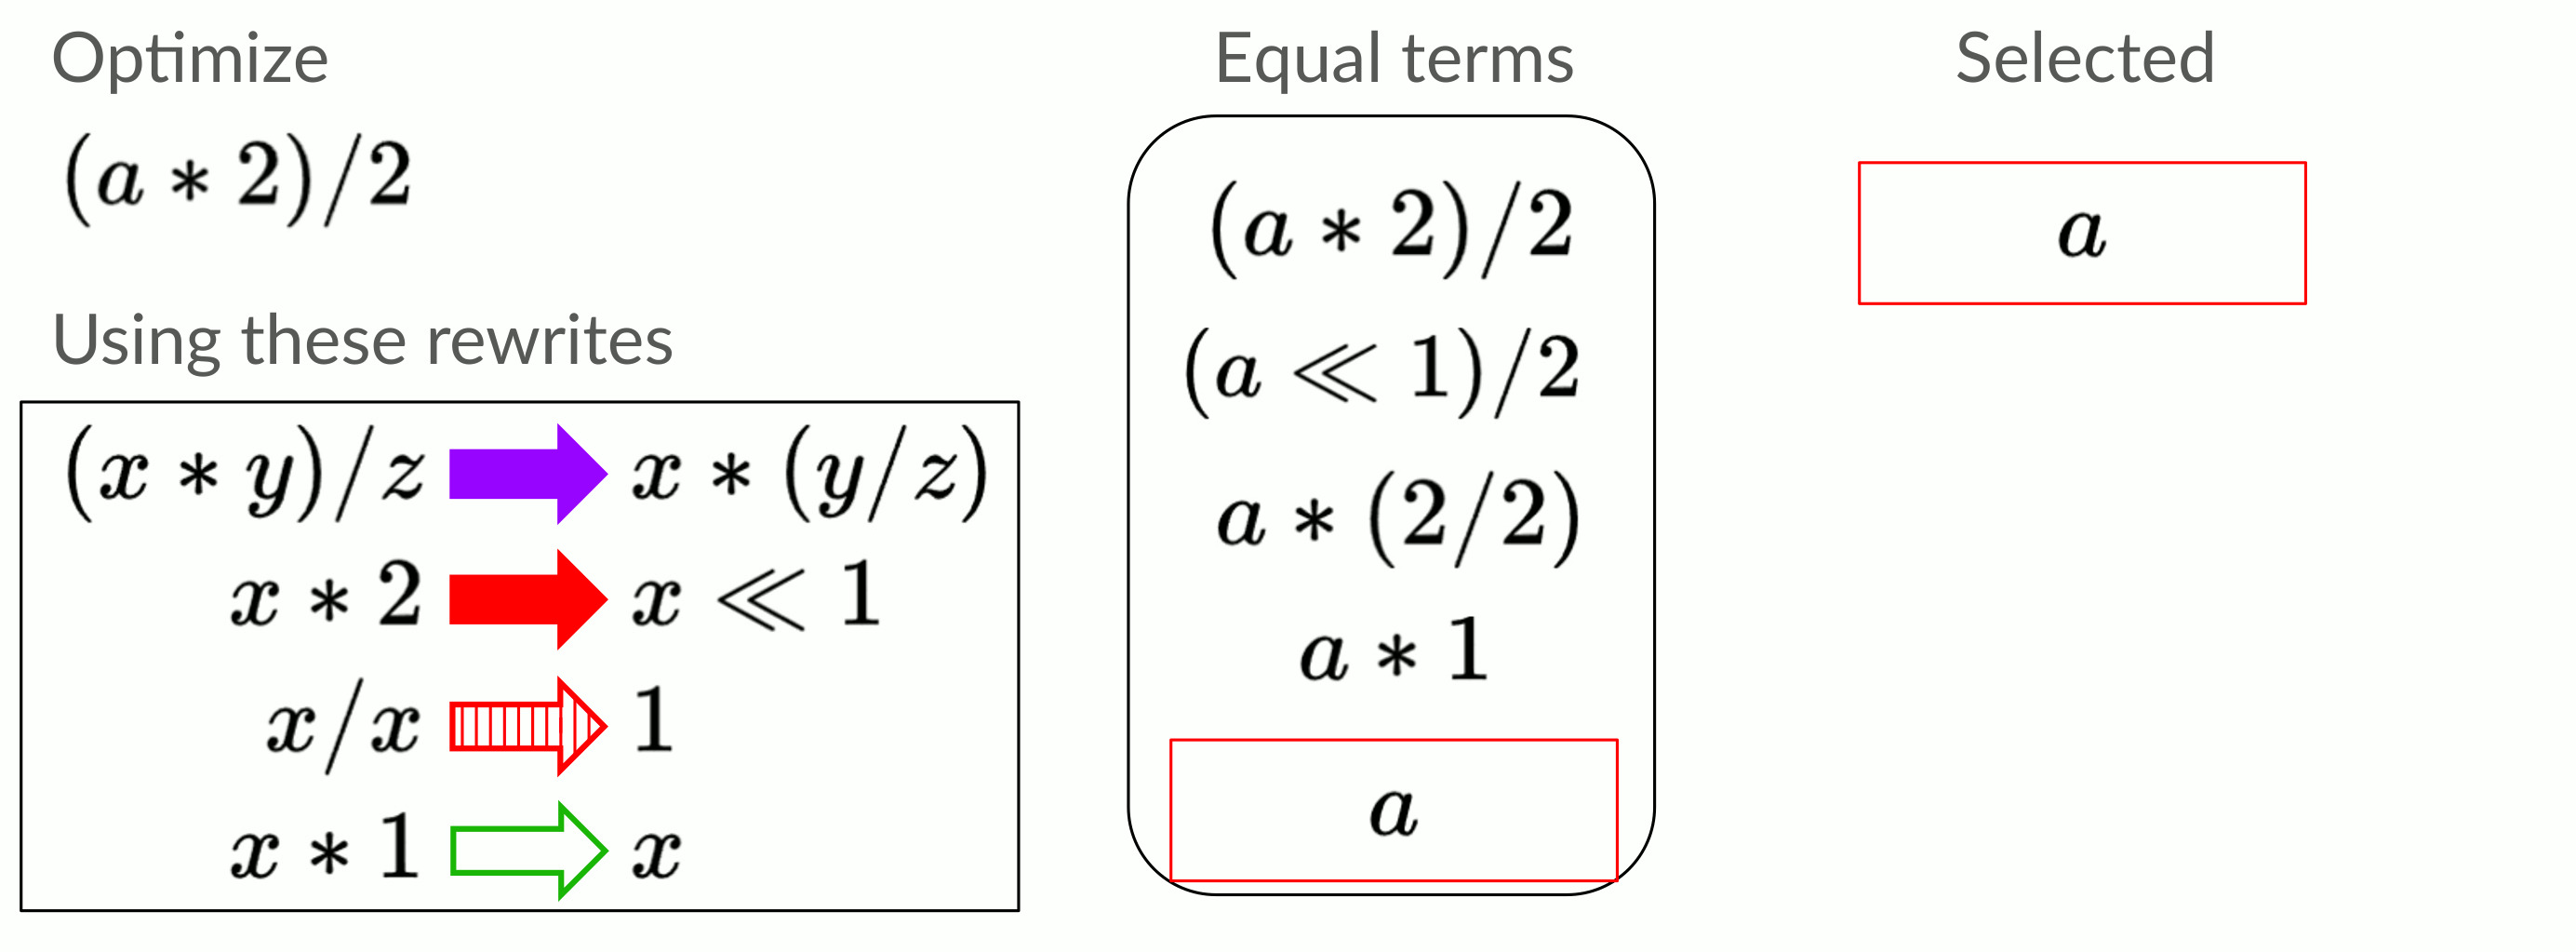
\includegraphics[width=13cm, height=5cm]{misc/egraphs_images/naive/n-14.jpg}
   }
   \only<16>
    {
        \centering
        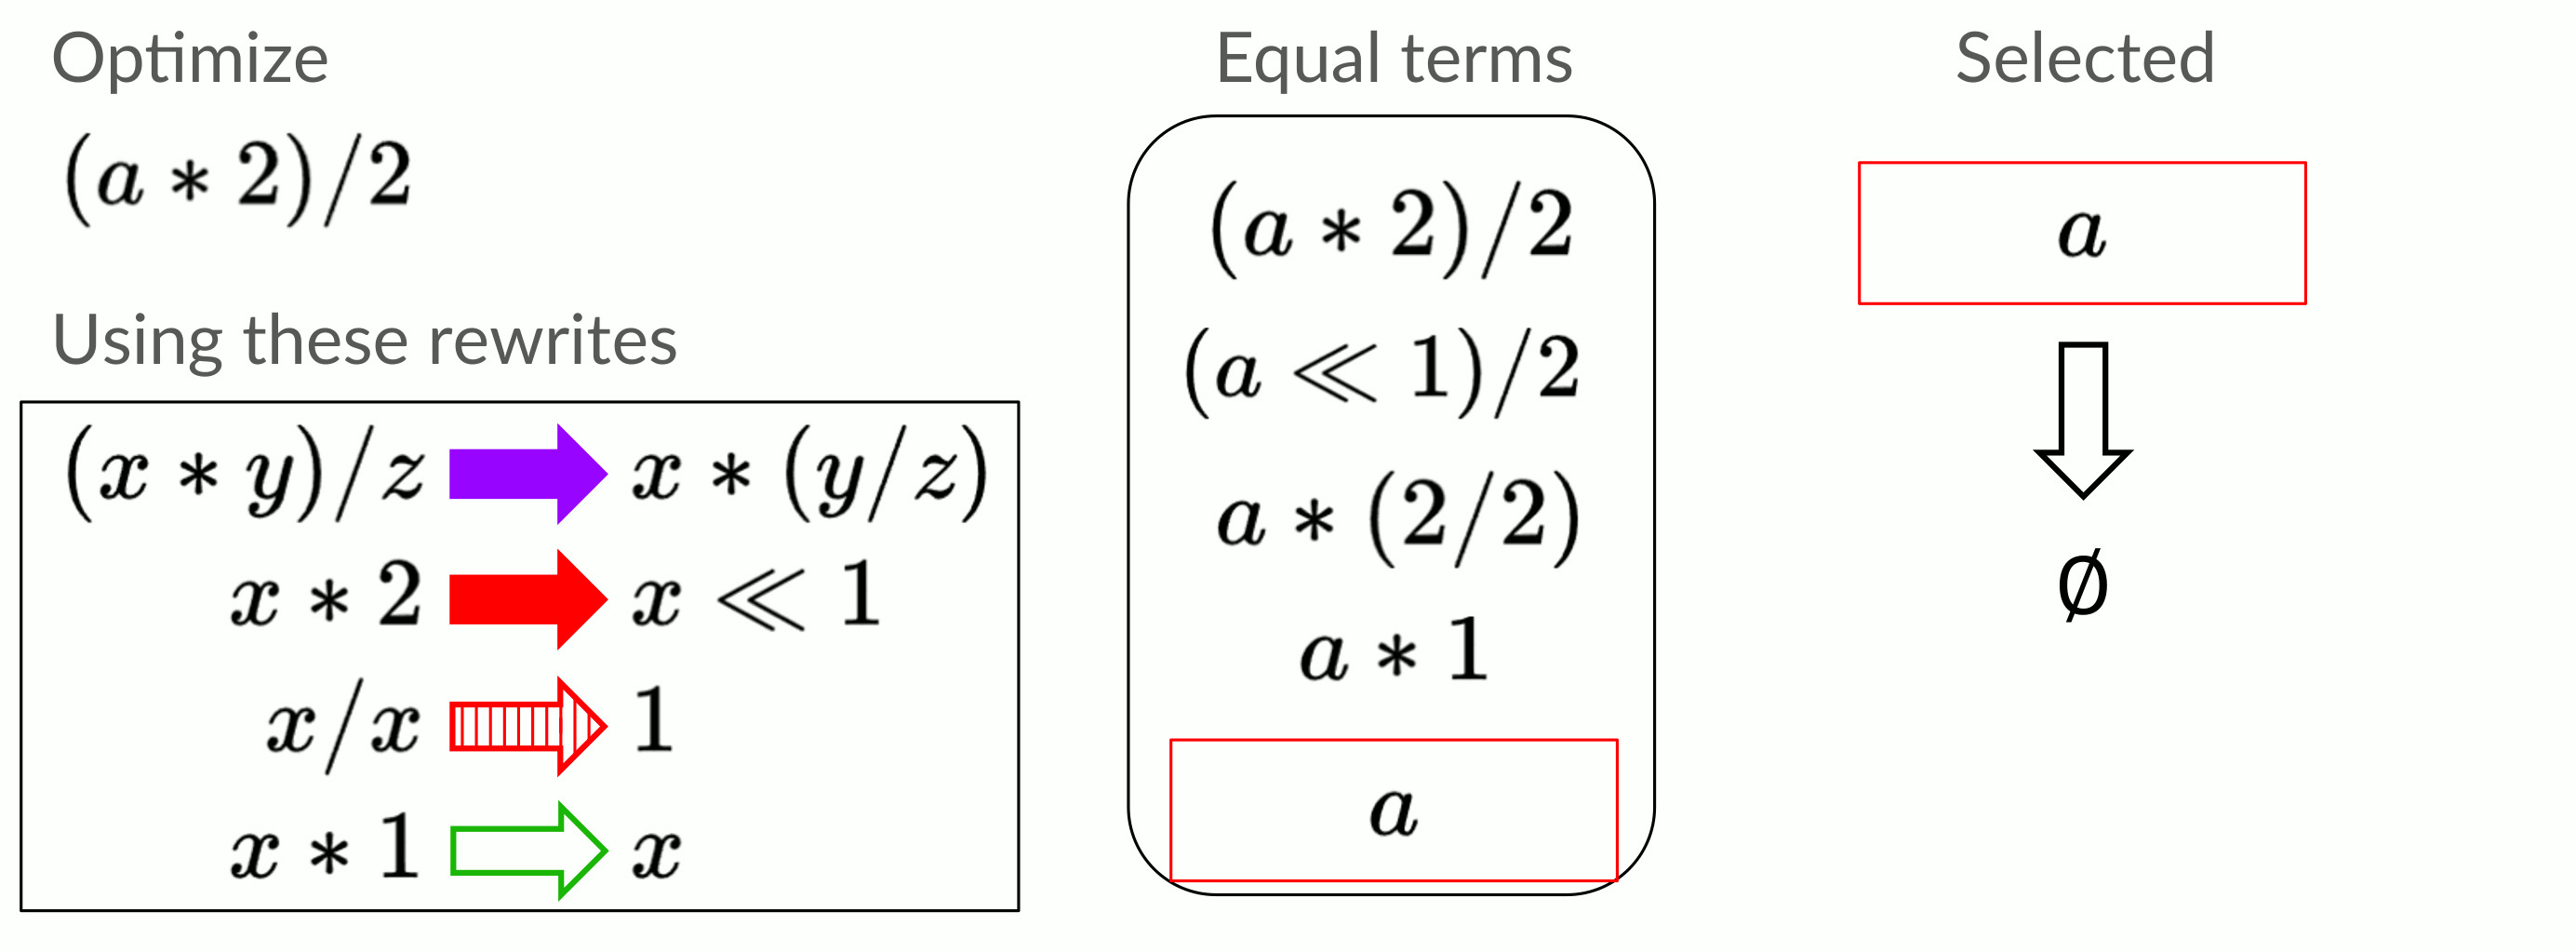
\includegraphics[width=13cm, height=5cm]{misc/egraphs_images/naive/n-15.jpg}
   }
   \only<17>
    {
        \centering
        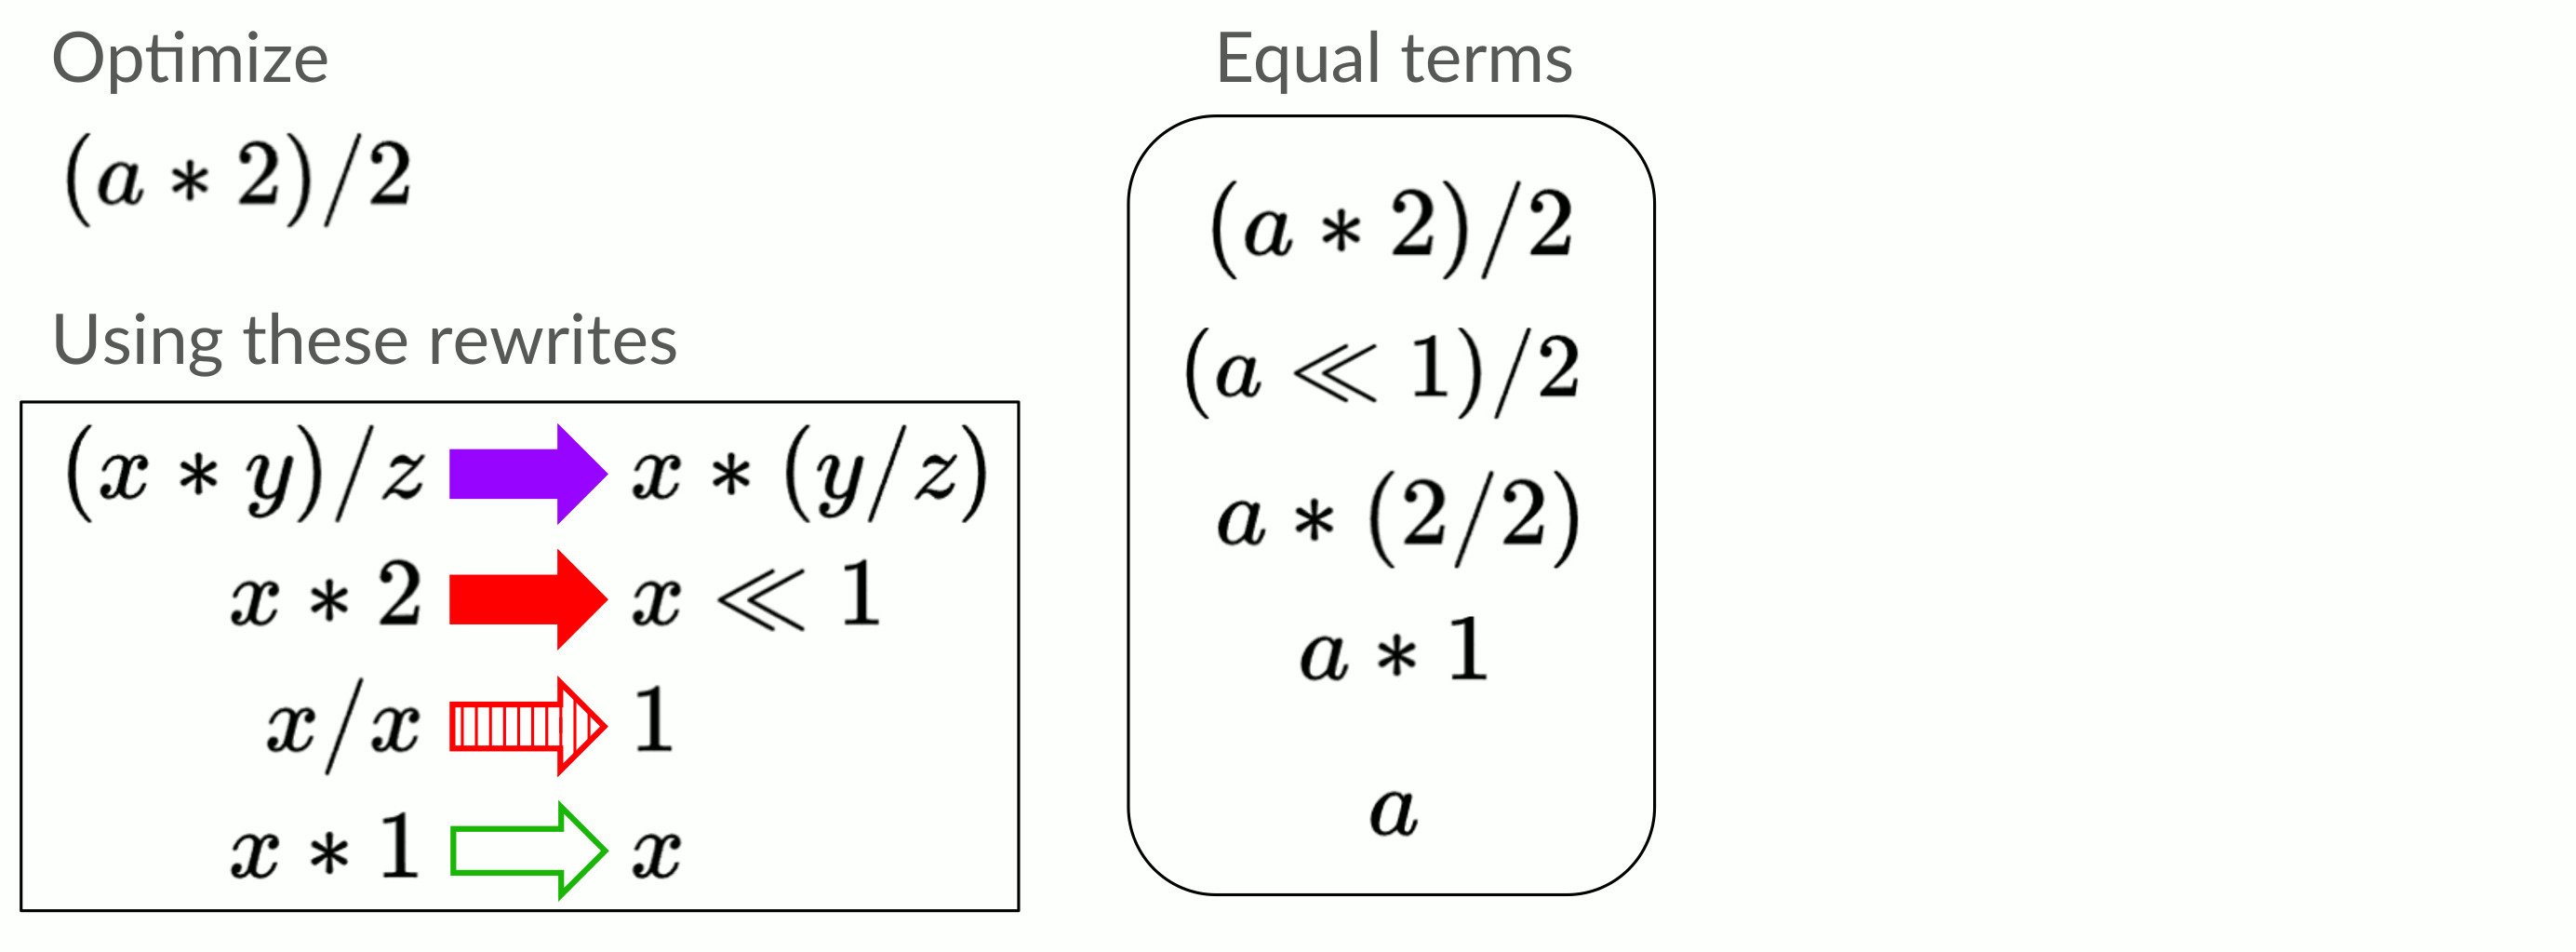
\includegraphics[width=13cm, height=5cm]{misc/egraphs_images/naive/n-16.jpg}
   }
\end{frame}

\begin{frame}{Решение проблемы 2/3}
    \begin{center}
            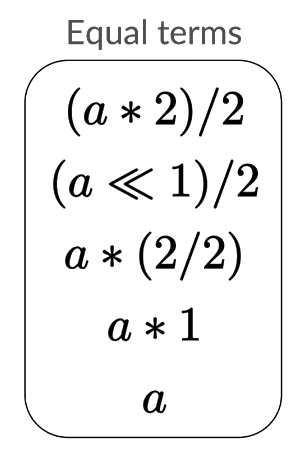
\includegraphics[width=3.2cm, height=4.2cm]{misc/egraphs_images/1_11new.png}
            \hspace{0.5cm}
            \raisebox{11.5ex}{$\xrightarrow{\text{\fontsize{10.0}{12} $a = b$}}$}
            \hspace{0.5cm}
            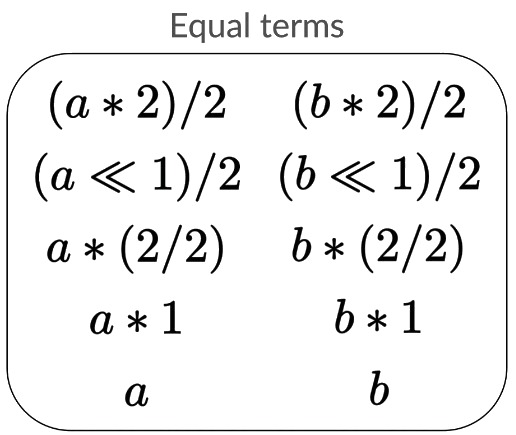
\includegraphics[width=5.2cm, height=4.2cm]{misc/egraphs_images/1_22new.jpg}
    \end{center}
\end{frame}

\begin{frame}{Решение проблемы 2/3}
    \centering
        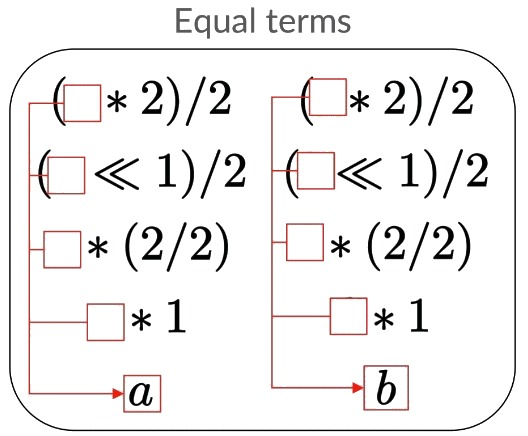
\includegraphics[width=8cm, height=5cm]{misc/egraphs_images/shared_im.jpg}
\end{frame}

\begin{frame}{Решение проблемы 3/3}
    \centering
        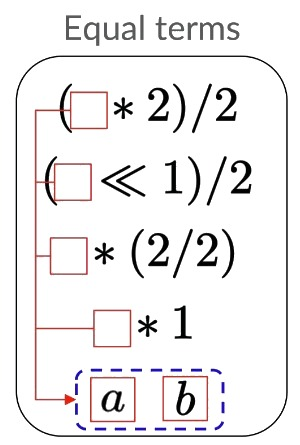
\includegraphics[width=5cm, height=6cm]{misc/egraphs_images/eclass_new.jpg}
\end{frame}





\begin{frame}{E-Graphs}
    \begin{block}{Определение}
        E-Graph --- это структура данных, предназначенная для хранения отношений эквивалентности над выражениями некоторого языка.
    \end{block}

    \begin{columns}
        \begin{column}{0.5\textwidth}
            \centering
            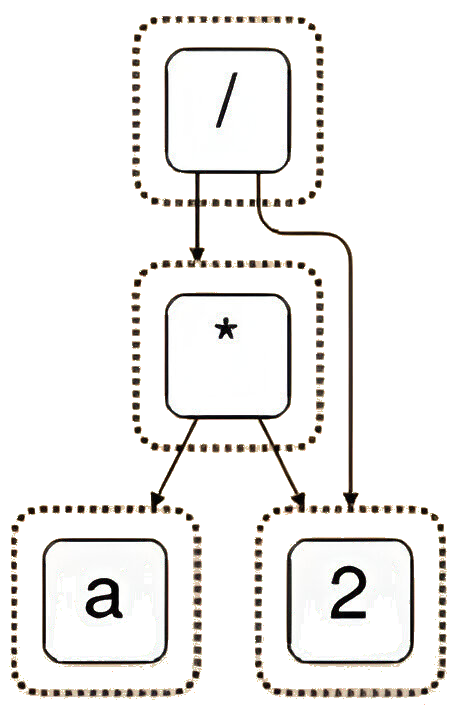
\includegraphics[width=5cm, height=5cm]{misc/egraphs_images/egraph_1.png} % Left middle image
        \end{column}
        \begin{column}{0.5\textwidth}
            \centering
            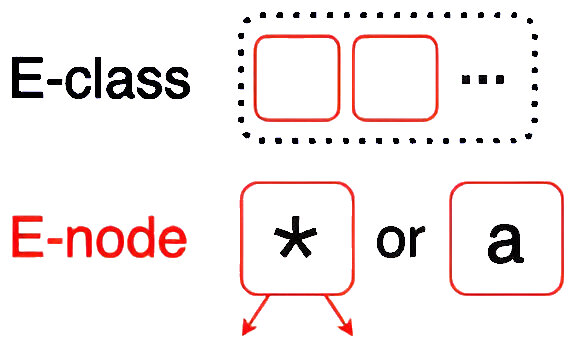
\includegraphics[width=5.2cm, height=4.2cm]{misc/egraphs_images/enodes_eclasses.jpg} % Right middle image
        \end{column}
    \end{columns}

\end{frame}

\begin{frame}{E-Graph. Насыщение 1/3}
    \only<1>
    {
        \begin{center}
            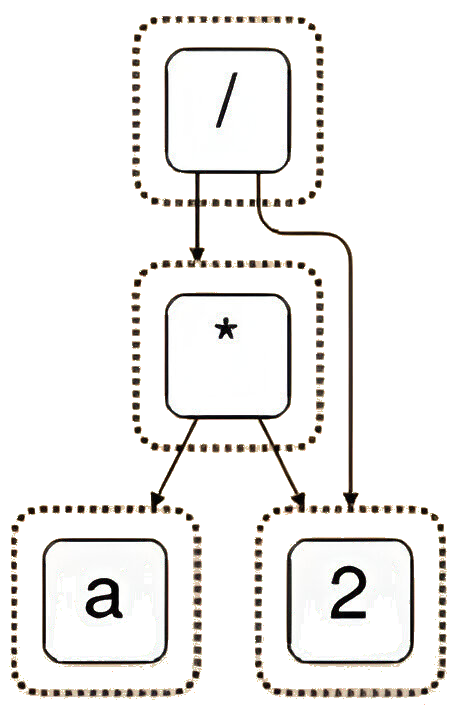
\includegraphics[width=5.2cm, height=4.2cm]{misc/egraphs_images/egraph_1.png}
        \end{center}
    }
    \only<2>
    {
        \begin{center}
            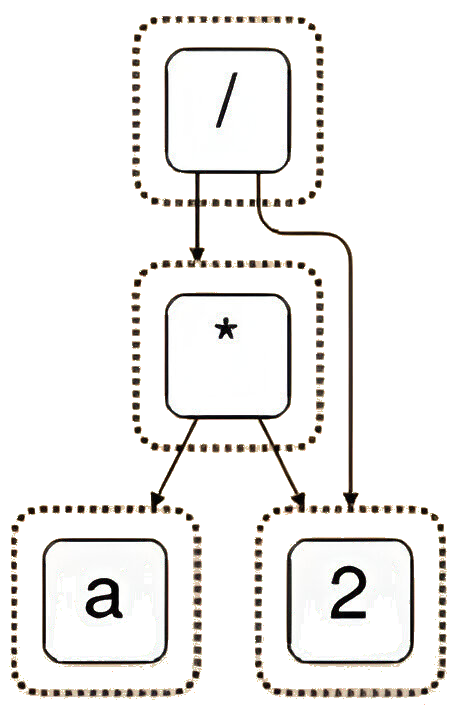
\includegraphics[width=5.2cm, height=4.2cm]{misc/egraphs_images/egraph_1.png}
            \hspace{0.5cm}
            \raisebox{11.5ex}{$\xrightarrow{\text{\fontsize{10.0}{12} $x\; * \;2 \; = \; x \; << \; 1$}}$}
            \hspace{0.5cm}
            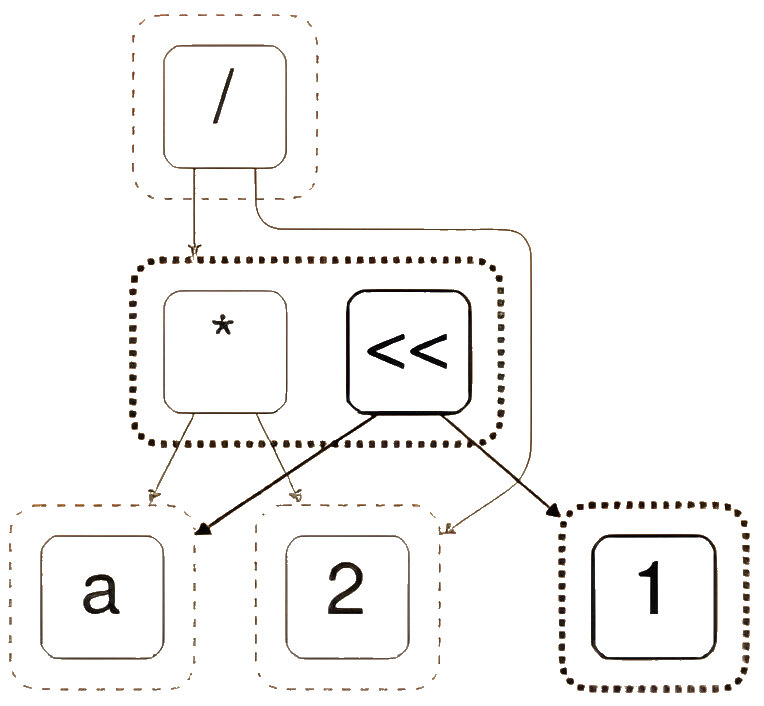
\includegraphics[width=5.2cm, height=4.2cm]{misc/egraphs_images/egraph_2.jpg}
        \end{center}
    }
\end{frame}

\begin{frame}{E-Graph. Насыщение 2/3}
    \only<1>
    {
        \begin{center}
            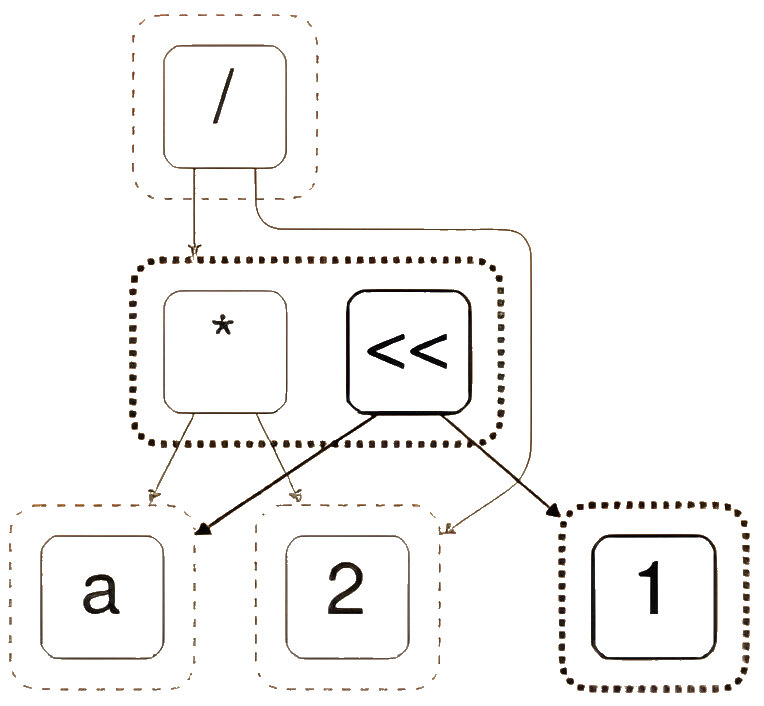
\includegraphics[width=5.2cm, height=4.2cm]{misc/egraphs_images/egraph_2.jpg}
        \end{center}
    }
    \only<2>
    {
        \begin{center}
            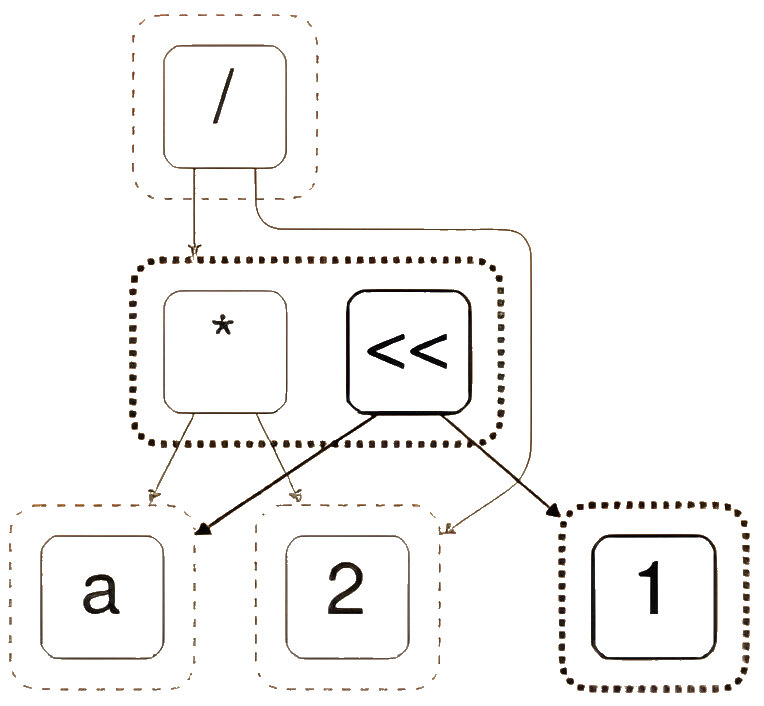
\includegraphics[width=5.2cm, height=4.2cm]{misc/egraphs_images/egraph_2.jpg}
            \hspace{0.5cm}
            \raisebox{11.5ex}{$\xrightarrow{\text{\fontsize{9.4}{12} $(x*y)/z = x*(y/z)$}}$}
            \hspace{0.5cm}
            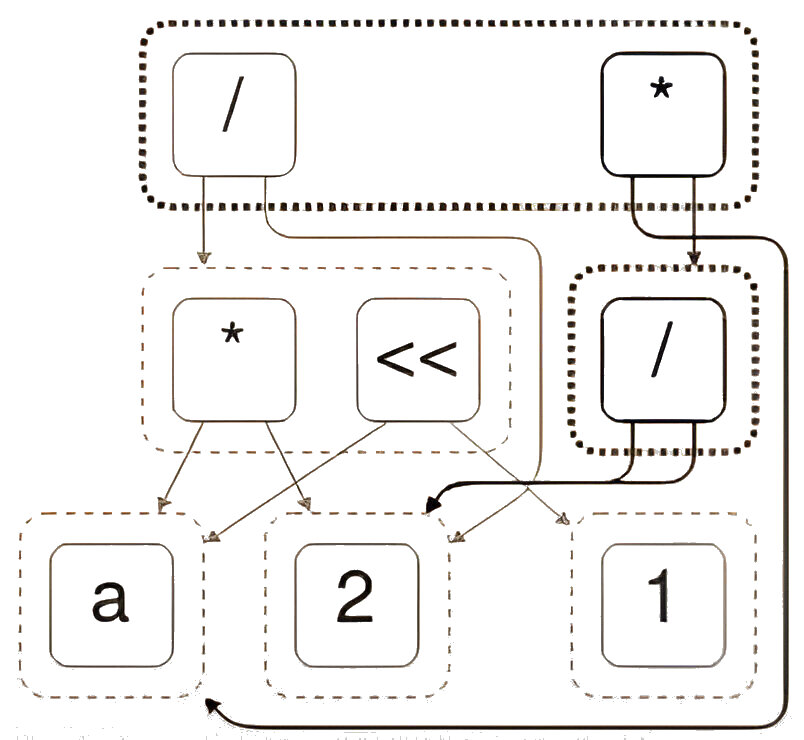
\includegraphics[width=5.2cm, height=4.2cm]{misc/egraphs_images/egraph_3.jpg}
        \end{center}
    }
\end{frame}

\begin{frame}{E-Graph. Насыщение 3/3}
    \only<1>
    {
        \begin{center}
            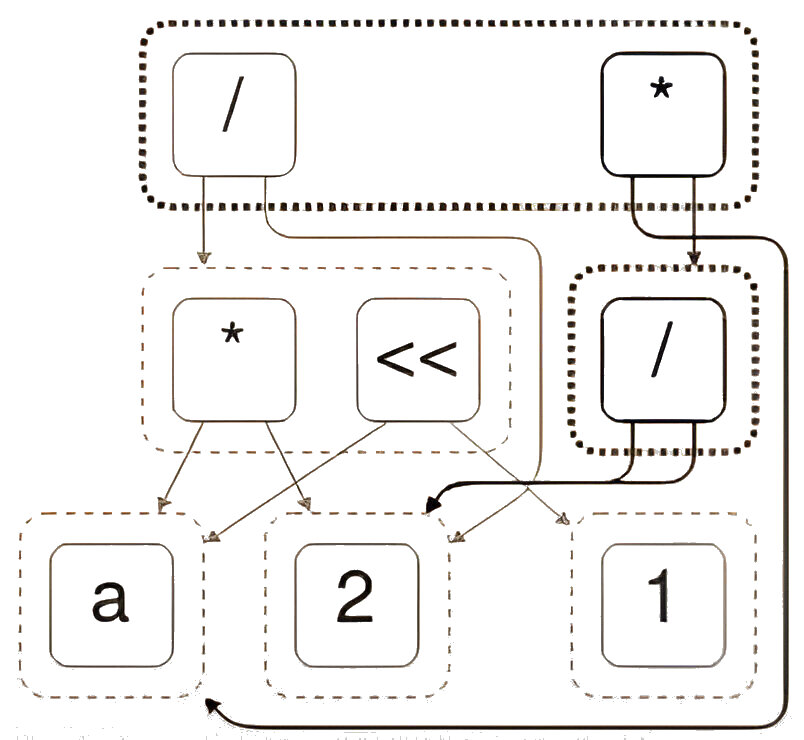
\includegraphics[width=5.2cm, height=4.2cm]{misc/egraphs_images/egraph_3.jpg}
        \end{center}
    }
    \only<2>
    {
        \begin{center}
            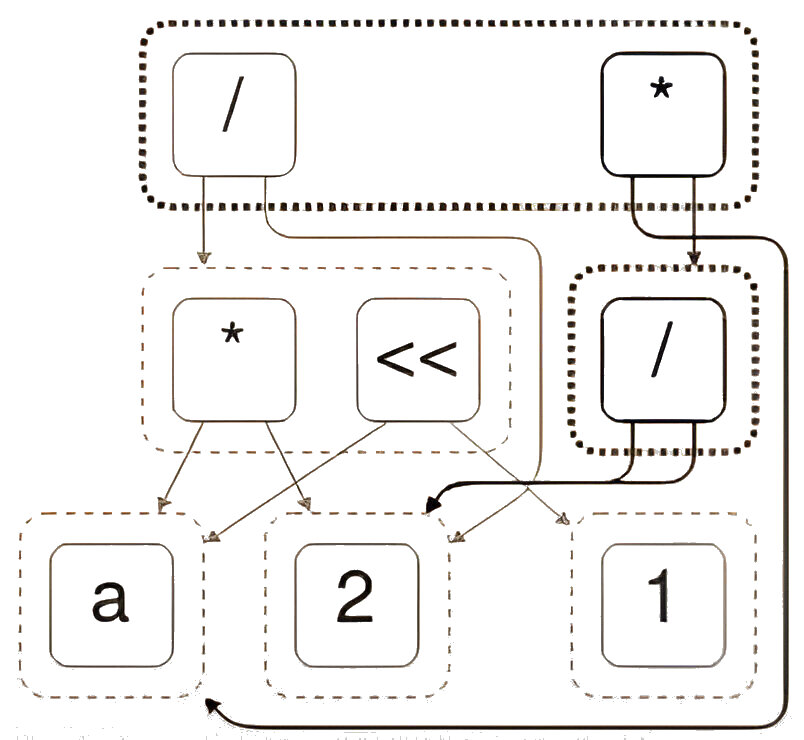
\includegraphics[width=5.2cm, height=4.2cm]{misc/egraphs_images/egraph_3.jpg}
            \hspace{0.5cm}
            \raisebox{11.5ex}
            {$\xrightarrow[\text{\fontsize{10.4}{12} $x / x = 1$}]{\text{\fontsize{10.4}{12} $x * 1 = x$}}$}
            \hspace{0.5cm}
            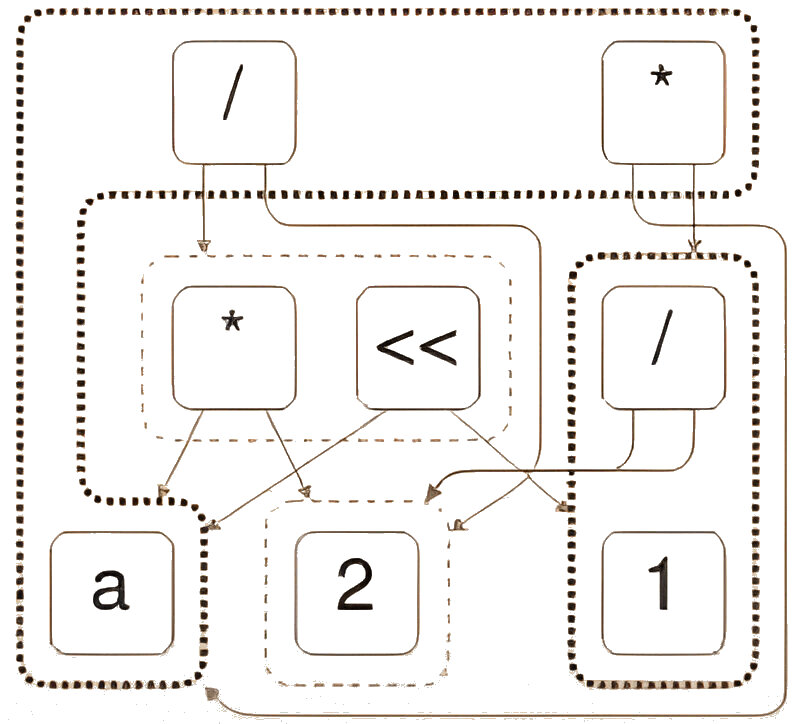
\includegraphics[width=5.2cm, height=4.2cm]{misc/egraphs_images/egraphs4.jpg}

        \end{center}

        \begin{center}
           \textbf{Так же содержит циклы, $a * 1$, $a * 1 * 1$ ...} \\
        \end{center}

    }
\end{frame}

\begin{frame}{Equality saturation}
    \begin{center}
        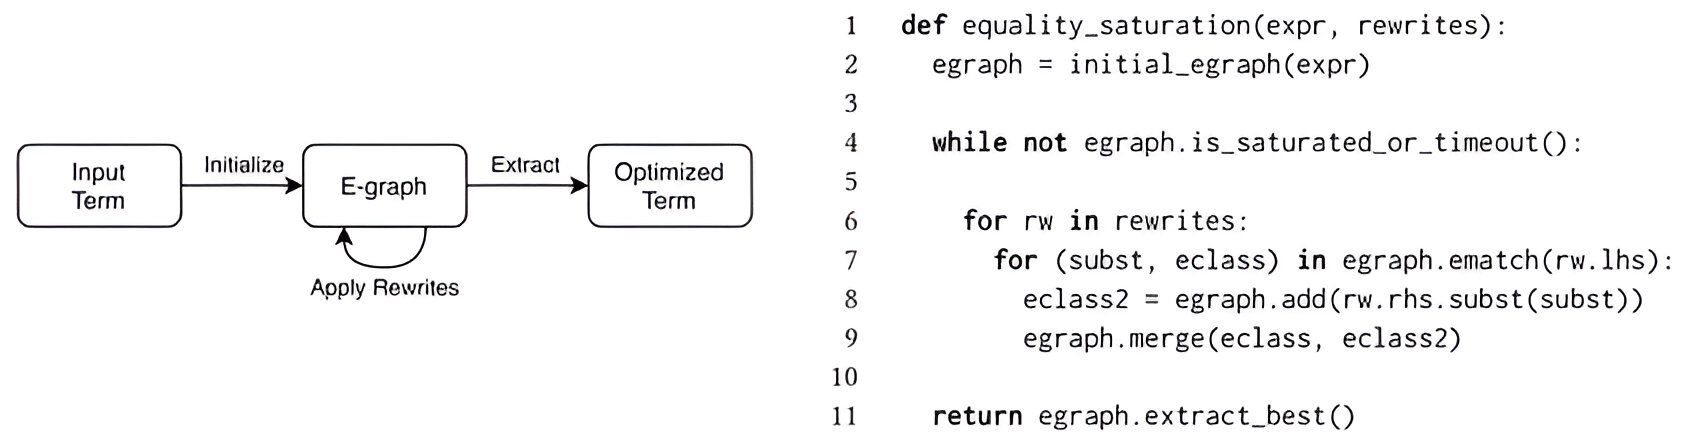
\includegraphics[width=15.2cm, height=5.2cm]{misc/egraphs_images/equality_saturation1.jpeg}
    \end{center}

    \begin{center}
       \begin{itemize}
           \item \textbf{Инвариант: если $a = b$, то $f(a) = f(b)$} \\
           \item \textbf{Извлечение} --- NP-complete проблема \\
       \end{itemize}


    \end{center}
\end{frame}

\begin{frame}{E-graphs Community}
    \begin{itemize}
        \item \textbf{egg} (\textbf{eg}raphs \textbf{g}ood)\textit{ $-$ A flexible, high-performance e-graph library} (Rust)\newline
        \item \textbf{Ego} (\textbf{Eg}raphs in \textbf{O}Caml) $-$ Библиотека для работы с е-графами и equality saturation в общих чертах повторяющая дизайн egg (OCaml)\newline

        \textbf{demo}

    \end{itemize}
\end{frame}

\begin{frame}{}
    \centering
    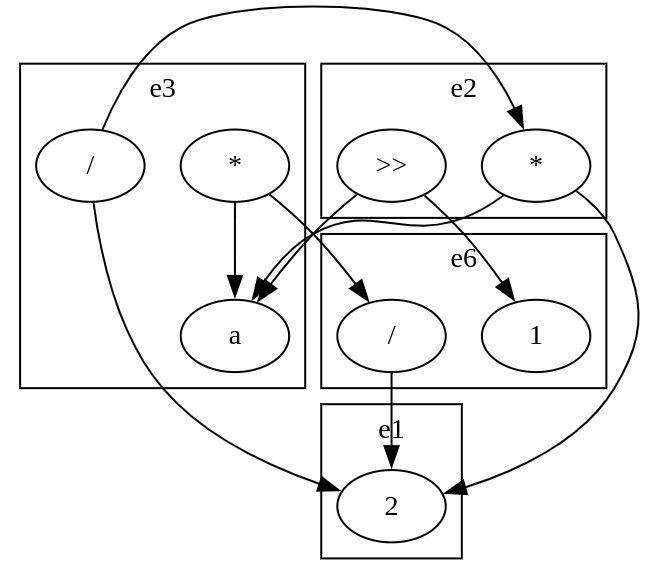
\includegraphics[width=10.2cm, height=7.2cm]{misc/egraphs_images/demo_egraph.jpeg}
\end{frame}

\begin{frame}{}
    \centering
    \textbf{\Huge Примеры оптимизаций, выразимых с E-Graphs} \\
    \vspace{1cm}
\end{frame}

\begin{frame}{Algebraic Simplifications}
    \begin{itemize}
    \item \textbf{\fontsize{14.1}{12} Нейтральный элемент по сложению:} \textbf{\fontsize{14.1}{12} $a + 0 = a$}
    \item \textbf{\fontsize{14.1}{12} $0 + a = a$}
    \newline
    \item \textbf{\fontsize{14.1}{12} Нейтральный элемент по умножению:} \textbf{\fontsize{14.1}{12} $a \cdot 1 = a$}
    \item \textbf{\fontsize{14.1}{12} $1 \cdot a = a$}
    \newline
    \item \textbf{\fontsize{14.1}{12} Обратный элемент по умножению:} \textbf{\fontsize{14.1}{12} $a \cdot 0 = 0$}
    \item \textbf{\fontsize{14.1}{12} $0 \cdot a = 0$}
    \newline
    \item \textbf{\fontsize{14.1}{12} Нейтральный элемент по делению:} \textbf{\fontsize{14.1}{12} $a \; / \; 1 = a$}
    \newline
    \item \textbf{\fontsize{14.1}{12} ...}
\end{itemize}
\end{frame}

\begin{frame}{}
    \centering
    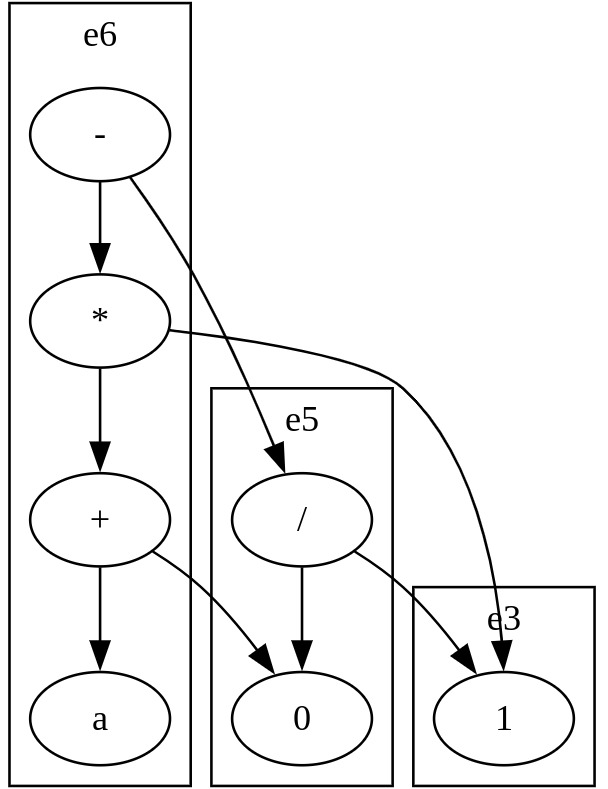
\includegraphics[width=10.2cm, height=7.2cm]{misc/egraphs_images/algebraic_simpl_demo.jpeg}
\end{frame}

\begin{frame}{Strength reduction}
    \begin{itemize}
    \item \textbf{\fontsize{14.1}{12} Умножение на степень двойки:} \textbf{\fontsize{14.1}{12} $a \; * \; 2^n = a << n$}
    \newline
    \item \textbf{\fontsize{14.1}{12} Деление на степень двойки:} \textbf{\fontsize{14.1}{12} $a \; / \;  2^n = a >> n$}
    \newline
    \item \textbf{\fontsize{14.1}{12} Проверка четности:} \textbf{\fontsize{14.1}{12} $x \; \% \; 2 = x \; \& \; 1$}
    \newline
    \item \textbf{\fontsize{14.1}{12} ...}
\end{itemize}
\end{frame}

\begin{frame}{}
    \centering
    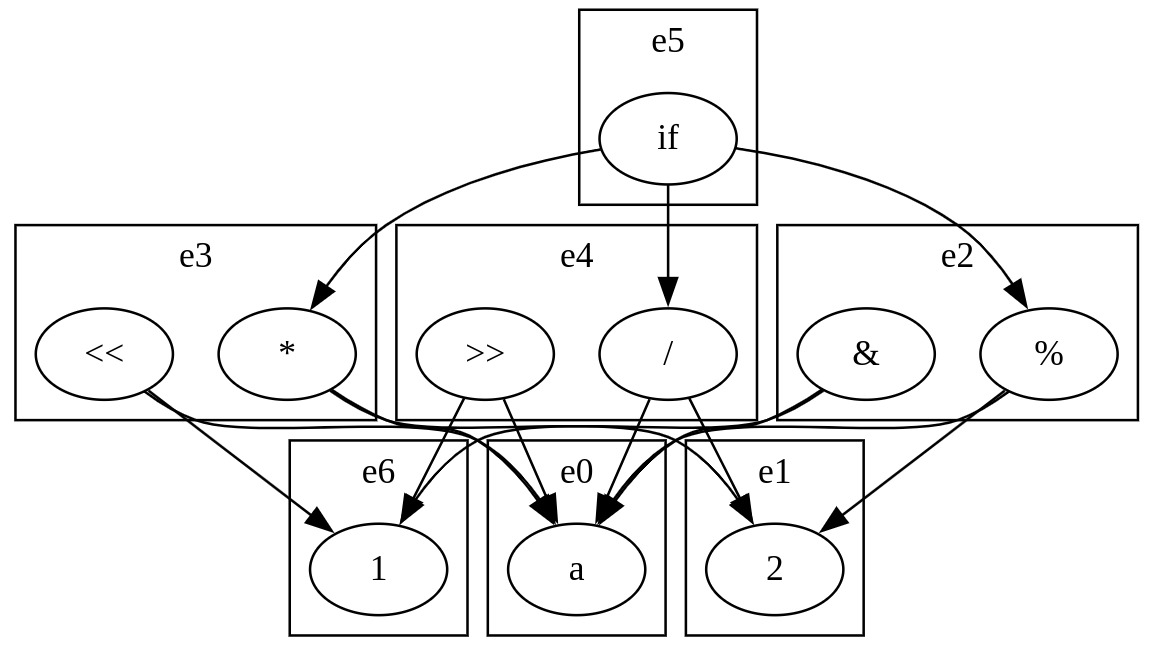
\includegraphics[width=10.2cm, height=7.2cm]{misc/egraphs_images/strength_red.jpeg}
\end{frame}

\begin{frame}{Function inlining}
    \begin{itemize}
    \item \textbf{\fontsize{14.1}{12} Замена вызовов функции непосредственно её телом}

\end{itemize}
\end{frame}

\begin{frame}{}
    \centering
    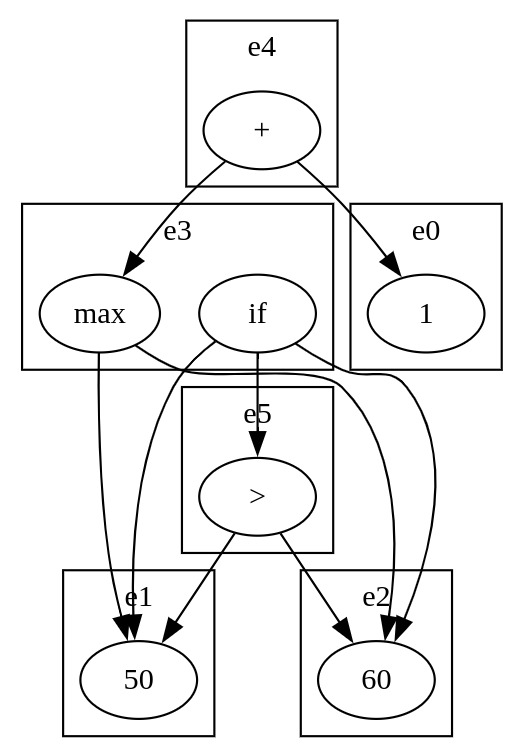
\includegraphics[width=7.2cm, height=7.2cm]{misc/egraphs_images/inlining_demo.jpeg}
\end{frame}

\begin{frame}{Common subexpression elimination}
    \centering
    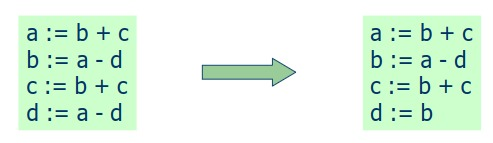
\includegraphics[width=12.2cm, height=5.2cm]{misc/egraphs_images/cse.jpeg}
\end{frame}

\begin{frame}{}
    \centering
    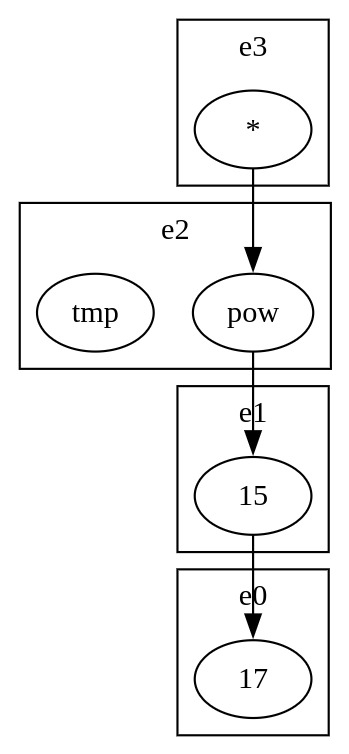
\includegraphics[width=4.2cm, height=6.2cm]{misc/egraphs_images/cse_demo.jpeg}
\end{frame}

\begin{frame}{Прочие оптимизации}
    \begin{itemize}
    \item \textbf{\fontsize{14.1}{12} Constant folding \& Constant propagation }
    \newline
    \item \textbf{\fontsize{14.1}{12} CSE for Arrays (Удаление избыточного доступа к массиву) }
    \newline
    \item \textbf{\fontsize{14.1}{12}  Loop Peeling (Вытаскиваем первую итерацию цикла)}
    \newline
    \item \textbf{\fontsize{14.1}{12}  Tail-call elimination}
    \newline
    \item \textbf{\fontsize{14.1}{12}  ...}
    \newline
    \end{itemize}
\end{frame}

\begin{frame}{Equality saturation \& E-Graphs. Pros and cons}
    \begin{columns}
        \column{0.5\textwidth}
        \textbf{Приемущества}
        \begin{itemize}
            \item \textbf{Выразимость}
            \item \textbf{Инкрементальное обновление}
            \item \textbf{Оптимальность}
        \end{itemize}

        \column{0.5\textwidth}
        \textbf{Недостатки}
        \begin{itemize}
            \item \textbf{Memory usage}
            \item \textbf{Perfomance overhead (слияние нодов)}
            \item \textbf{NP-полнота извлечения}
        \end{itemize}
    \end{columns}
\end{frame}

\begin{frame}{Где ещё можно встретить e-graphs?}
    \begin{itemize}
    \item \textbf{\fontsize{14.1}{12} Theorem provers (Lean) \cite{Lean}}
    \newline
    \item \textbf{\fontsize{14.1}{12} Deep learning (Graph rewriting)\cite{Deep_learning}}
    \newline
    \item \textbf{\fontsize{14.1}{12} SMT-solvers\cite{CMT} }
    \newline
    \item \textbf{\fontsize{14.1}{12} ... }
    \end{itemize}
\end{frame}

\begin{frame}{Вопросы}
    \begin{itemize}
    \item \textbf{\fontsize{14.1}{12} 1. Переписывние выражений. Правила переписывания. Полезные и бесполезные правила. Примеры. }
    \newline
    \item \textbf{\fontsize{14.1}{12}
2. E-графы. Equality saturation. Примеры оптимизаций выразимых с помощью equality saturation и е-графов.}
    \newline
    \item \textbf{\fontsize{14.1}{12} 3. Изобразить е-граф для выражения $(a + 0) + (a * 1)$ и примененить к нему следующие правила: $a + 0 = a$, $a * 1 = a$ }
    \newline
    \item \textbf{\fontsize{14.1}{12} 4. Приемущества и недостатки equality saturation и e-графов
 }
    \end{itemize}
\end{frame}

\begin{frame}%[allowframebreaks]
\frametitle<presentation>{Ссылки \& Acknowledgements}
\phantom{\cite*{Deep_learning,CMT,Lean}}
\vspace{-1em}
\printbibliography
\end{frame}


\end{document}
